% Main file — compile with pdflatex (or use Overleaf).
% Default class: article with twocolumn. Swap in ACL/EMNLP .sty later.

\documentclass[11pt,a4paper]{article}
\usepackage[hmargin=2cm,vmargin=2.5cm]{geometry}
\usepackage{cmap}              % must precede fontenc; fixes PDF text-layer
                               % so copy/paste and pdftotext preserve spaces
\usepackage[T1]{fontenc}
\usepackage[utf8]{inputenc}
\usepackage{lmodern}           % cleaner glyph-to-Unicode mapping than default CM
\usepackage{microtype}
\usepackage{amsmath,amssymb}
\usepackage{booktabs}
\usepackage{graphicx}
\usepackage{xcolor}
\usepackage{url}
\usepackage[hidelinks]{hyperref}
\usepackage{cite}
\usepackage{caption}
\captionsetup{font=small, labelfont=bf}

% Single-column for now (easier to draft). Switch to twocolumn for final.
% \twocolumn

\title{Data Quality and Model Capacity in Transformer MT:\\
  A Two-by-Two Controlled Ablation}
\author{
  Jizheng Huang \\
  University of Toronto \\
  \texttt{jizheng.huang@mail.utoronto.ca}
}
\date{\today}

\begin{document}
\maketitle

\begin{abstract}
Does extra Transformer capacity always pay? We probe the data-quality/capacity interaction with a controlled two-by-two ablation on WMT14 en-fr: (strict-filter 9.3M vs.\ loose-filter 30M) x (Base 60M vs.\ Big 209M), trained from scratch on a shared source pool, SPM, and pipeline. \textbf{Under this data regime, the capacity return changes sign with data quality}: on clean data Big exceeds Base by $+0.56$ test BLEU; on noisy data Big falls below Base by $-0.87$. The pattern replicates on WMT14 en-de at 4.5M scale, where Big falls below Base by $-1.57$ BLEU on newstest2014. As a post-training follow-up, we test whether continued training on a QE-filtered subset (top-1M by CometKiwi-22~\cite{rei2022cometkiwi}; cross-entropy fine-tuning, not instruction or preference tuning) recovers the loose-corpus deficit. It does not: both models degrade by 1.5--2.3 BLEU, because the QE-top of a multi-domain corpus is heavily UN/legislative --- high-quality, but mismatched to news-domain newstest. We argue that this decomposes ``data quality'' into translation correctness and alignment to the eval distribution --- two independent axes, of which reference-free QE measures only the first. The unifying claim is that \emph{capacity acts as a force multiplier whose sign depends on the supervision signal it is multiplying}, whether that signal is wrong-because-noisy (\S\ref{sec:enfr_v2}) or wrong-because-mismatched (\S\ref{sec:sft}). All code, four published checkpoints, and stdout logs are released.

\end{abstract}

\section{Introduction}

The Transformer~\cite{vaswani2017attention} is the most-cited baseline in machine translation, and its WMT14 numbers --- 27.3 tokenized BLEU for Base on en-de, 38.1 for Big on en-fr --- are the reference point against which post-2017 progress is measured. Reproducing those numbers is harder than the paper's compactness suggests: tokenized BLEU is not directly comparable to modern sacrebleu~\cite{post2018call}, the preprocessing pipeline is under-specified, and the original 8-GPU training configuration no longer matches the typical reproduction environment of a single accelerator. Most work citing the Transformer paper quotes the numbers without re-running them. We re-run them on a single RTX 5090 and use the resulting infrastructure to ask a sharper question.

\paragraph{The question.}
Modern empirical ML has converged on two largely independent levers for improving a learning system: \emph{more capacity}~\cite{kaplan2020scaling, hoffmann2022chinchilla} and \emph{more, cleaner data}~\cite{penedo2023refinedweb, gururangan2020dont}. A common assumption is that pulling either lever, while holding the other roughly fixed, yields monotone gains. Our study challenges that assumption in a sharp form. On WMT14 en-fr, scaling Base (60M) to Big (209M) \textbf{changes sign as a function of data quality}: on a strictly-filtered 9.3M corpus, Big beats Base by $+0.56$ BLEU; on a loosely-filtered 30M corpus drawn from the same source pool, Big falls below Base by $-0.87$ BLEU. Under this controlled setup --- shared source pool, SPM, and pipeline --- a single architectural intervention pays in one regime and costs in another, with the regime determined by data quality.

\paragraph{What we do.}
We construct a controlled two-by-two design: data quality (strict-filter v1, loose-filter v2) x model capacity (Base, Big), and report all four from-scratch results on a single-GPU pipeline. We extend the design with cross-language replication (WMT14 en-de, where Big falls below Base by $-1.57$ BLEU on newstest2014 at 4.5M scale) and a post-training intervention: cross-entropy fine-tuning on a QE-filtered subset (top-1M of the noisy 30M, scored by CometKiwi-22~\cite{rei2022cometkiwi}; not instruction or preference tuning). The fine-tuning outcome is a clean negative finding that tightens the central claim: data quality is not a single number. It decomposes into translation correctness \emph{and} alignment to the eval distribution, and naive top-K-by-QE filtering optimizes only the first.

\paragraph{Contributions.}
\begin{enumerate}
\item A 2x2 ablation establishing that capacity return is sign-conditioned on data quality ($+0.56$ BLEU on clean data, $-0.87$ on noisy data, shared en-fr corpus pool, SPM, and pipeline; replicated qualitatively on en-de).
\item A post-training negative result showing that QE-filtered fine-tuning, at scale, degrades newstest BLEU by 1.5--2.3, with the larger model degrading more. The failure is mechanistically distinct from the pretraining-on-noise failure of \S\ref{sec:enfr_v2}, yet converges to the same 33--34 BLEU ceiling --- suggesting that incorrect supervision of \emph{any} form bounds achievable test accuracy by roughly the same amount.
\item A reproducible single-GPU Transformer pipeline that reaches 35.31 / 35.87 sacrebleu on WMT14 en-fr Base/Big and 24.04 on en-de Base, with open-source code, configurations, four published HuggingFace checkpoints, and persistent training logs. The full study reproduces in roughly 30 GPU-hours on a single 5090.
\item A methodology note on loss-spike-guard trigger rates as a diagnostic, with evidence that they cannot be read as a pure data-noise metric: under a fixed threshold the trigger rate is a joint function of data noise and the model's own convergence depth, so cross-capacity comparisons (Big on clean vs.\ Big on noisy) are confounded.
\end{enumerate}

\paragraph{Scope and limitations.}
We run single seeds per configuration. The variance of any individual BLEU number is unmeasured, but the $+0.56$ / $-0.87$ / $-1.55$ / $-2.33$ effects we make claims on are large relative to the typical Transformer-MT seed-variance band of ${\sim}0.2$--$0.4$ BLEU, and the cross-language replication supports the directional findings. We use sacrebleu 13a throughout and do not run human evaluation. We test only WMT14 en-fr and en-de; generalization to morphologically richer or non-Latin pairs (e.g., en-cs, en-ru, en-zh) is out of scope.

\paragraph{Roadmap.}
\S\ref{sec:related} reviews related work. \S\ref{sec:setup} describes the single-GPU setup. \S\ref{sec:enfr_v1}--\S\ref{sec:enfr_v2} present the en-fr v1 success and v2 failure runs that form the data-quality axis. \S\ref{sec:ende} extends the pattern to en-de. \S\ref{sec:sft} reports the QE-filtered fine-tuning negative result and the multi-dimensional view of ``data quality'' it implies. \S\ref{sec:methodology} is the methodology note on spike-guard interpretation. \S\ref{sec:conclusion} concludes.

\section{Related Work}
\label{sec:related}

\paragraph{Transformer reproduction.}
The original Transformer~\cite{vaswani2017attention} reports tokenized BLEU on WMT14 en-de (Base 27.3, Big 28.4) and en-fr (Big 41.0); subsequent re-implementations using sacrebleu~\cite{post2018call} typically land 1.5--2 BLEU lower in equivalent units, due to tokenizer and BLEU-variant differences~\cite{post2018call}. Our results (Base en-fr 35.31, Big en-fr 35.87, Base en-de 24.04 sacrebleu) sit within or above this expected band.

\paragraph{Scaling laws.}
\cite{kaplan2020scaling} and \cite{hoffmann2022chinchilla} establish that test loss scales as a power law in compute, parameters, and data. These laws assume data quality is held fixed across the scaling range; our 2x2 directly probes the quality--capacity interaction that the laws abstract away. The closest scaling-law observation we are aware of is~\cite{tay2022scaling}'s finding that data quality interacts with effective compute, but their setting is encoder-only and does not isolate the capacity sign-flip reported here.

\paragraph{Data curation for MT.}
Aggressive corpus filtering for MT is well studied~\cite{koehn2018findings, junczys2019cscope}, typically via length, language-ID, and parallelism heuristics, and increasingly via neural QE filters~\cite{batheja2022qe}. We use a strict v1 filter inspired by~\cite{gururangan2020dont}'s strict-DAPT setup, plus a CometKiwi-22~\cite{rei2022cometkiwi} top-K filter for fine-tuning. Our negative fine-tuning result is consistent with~\cite{junczys2019cscope}'s observation that domain-adaptive filtering can degrade out-of-domain BLEU even when filter quality is verifiable.

\paragraph{Loss-based sample selection.}
RHO-Loss~\cite{mindermann2022prioritized} uses model-relative loss to identify learnable samples; our spike-guard is mechanically simpler --- it drops high-loss batches via a $1.3\times$ EMA threshold --- and is intended for noise filtering, not curriculum design. \S\ref{sec:methodology} reports an unanticipated property of mechanisms of this kind: trigger rates are a joint function of data noise and model convergence depth, which complicates their use as a pure data diagnostic.

\section{Experimental Setup}
\label{sec:setup}

This section documents the single-GPU pipeline used to produce all subsequent results. The pipeline is released in full at \url{https://github.com/Euswbnix/Machine_translation} (pretraining) and \url{https://github.com/Euswbnix/Machine-Translation-SFT} (post-training).

\subsection{Hardware and software}
All training runs use a single NVIDIA RTX 5090 (Blackwell, sm\_120, 32~GB VRAM, 600~W TDP). Software stack: Python 3.10, PyTorch 2.8 nightly (CUDA 12.8 build for sm\_120), SentencePiece 0.1.99, sacrebleu 2.3, and CometKiwi-22 via \texttt{unbabel-comet 2.2}. We train in bf16 throughout (autocast); a brief fp16 attempt on Big diverged and was abandoned.

\subsection{Data}
\paragraph{WMT14 en-fr.} The raw parallel corpus contains $\sim$~40.8M sentence pairs (Europarl, News Commentary, Common Crawl, UN, Giga). We construct two cleaned variants from this same source:
\begin{itemize}
\item \textbf{v1 (strict, 9.3M).} The raw corpus is capped at 10M pairs (the first 10M from the HuggingFace Datasets stream, deterministic order), then cleaned with: empty/duplicate removal, length range [3, 200] tokens, src/tgt length ratio $\in [0.5, 2.0]$, and Latin-script ratio $\geq 0.9$. 9.3M pairs survive (93\% keep rate on the 10M head).
\item \textbf{v2 (loose, 30M).} The full 40.8M raw corpus, cleaned with identical per-pair filters but without the 10M cap. 30.1M pairs survive (74\% keep rate over all 40.8M; lower because the long tail beyond 10M contains more noisy or misaligned pairs).
\end{itemize}
The v1 / v2 split forms the data-quality axis of the 2x2 ablation: identical per-pair filters, different breadth.

\paragraph{WMT14 en-de.} Raw $\sim$~4.5M pairs (Europarl, News Commentary, Common Crawl). The same cleaning thresholds as v1 are applied (default settings of our cleaning script). 4.17M pairs survive (92.6\% keep rate; the en-de raw corpus is cleaner per-pair than en-fr).

\paragraph{Eval splits.} newstest2013 (3,000 pairs, valid) and newstest2014 (3,003 pairs, test) for both en-fr and en-de, downloaded via the WMT14 HuggingFace dataset.

\subsection{Tokenization}
SentencePiece BPE~\cite{sennrich2016neural, kudo2018sentencepiece}, joint en-fr (or en-de) vocabulary of 32{,}000 subwords, with \texttt{character\_coverage=1.0} so that accented characters (\textit{Israël}, \textit{Noël}, German umlauts) are not mapped to \texttt{<unk>}. The SPM is trained on the cleaned training corpus; valid and test sides reuse the same SPM. We share the input embedding, output embedding, and pre-softmax projection (Vaswani's \emph{tied embeddings} option).

\subsection{Model architectures}
We use the original Vaswani configurations. Base ($d_\text{model}{=}512$, $h{=}8$, $d_\text{ff}{=}2048$, $L{=}6{+}6$) totals 60.5M parameters with shared embeddings; Big ($d_\text{model}{=}1024$, $h{=}16$, $d_\text{ff}{=}4096$, $L{=}6{+}6$) totals 209M. Dropout is 0.1 throughout (en-fr), or 0.3 for en-de Big (following the original paper's stronger regularization for the smaller corpus). Maximum sequence length is 256 tokens.

\subsection{Training}
\paragraph{Optimization.} AdamW ($\beta_1{=}0.9$, $\beta_2{=}0.98$, $\epsilon{=}1\text{e-}9$), label-smoothed cross-entropy ($\alpha{=}0.1$), gradient clipping at $\|g\|{=}1.0$. Noam learning-rate schedule~\cite{vaswani2017attention} with $d_\text{model}^{-0.5}$ scale and a min-LR floor of $1\text{e-}5$ to prevent the late-Noam tail from approaching zero. Warmup 4K steps for Base / 8K for Big.

\paragraph{Effective batch.} We use token-based dynamic batching: each micro-batch packs $\leq$~24{,}576 tokens (Base) / 8{,}192 (Big), with $\leq$~192 / 64 sentences per micro-batch, and we accumulate 4 micro-batches per optimizer step. The effective batch is therefore $\sim$~98K tokens/step (Base) / 32K tokens/step (Big), matching the original paper's $\sim$~25K tok/batch on en-de once normalized by device count.

\paragraph{Run lengths.} Base v1.1 trains for 122K steps ($\sim$~3 epochs), Big v1.1 for 260K (early-stopped from a 280K plan), Base v2 for 600K, Big v2 for 416K (halted), Base en-de for 230K. Each Base run is $\sim$~2--3~h on the 5090; each Big run is $\sim$~6--7~h.

\paragraph{Loss-spike guard.} Each accumulated batch's average loss is compared against an EMA of recent batches (window $\alpha{=}0.005$, $\sim$~200 steps). If the current batch exceeds $1.3\times$ the EMA, the entire effective batch's gradient is discarded. The intent is to drop poisoned micro-batches without forcing a hard halt. Trigger counts are saved to the training report (\S\ref{sec:methodology}).

\paragraph{Adaptive eval interval.} Validation runs every 20K steps when the smoothed training loss is high (above 4.0) and every 2--3K steps once it crosses below 2.8, with linear interpolation in between. This avoids wasting compute on early-training BLEU evals (which are essentially noise) while keeping the late-training signal fine-grained.

\subsection{Evaluation}
\paragraph{BLEU.} sacrebleu 13a (default \texttt{intl} normalization, default \texttt{13a} tokenizer)~\cite{post2018call}. We report newstest2013 (valid) and newstest2014 (test). For en-de we additionally try the original paper's beam=4, length-penalty=0.6 setting (\S\ref{sec:ende}).

\paragraph{Decoding.} Beam search, beam size 5, length penalty 1.0 (en-fr) / 0.6 (en-de when comparing to the original paper), maximum decoded length 256.

\paragraph{Checkpoint averaging.} The classic Vaswani trick: average the parameters of the last 5 checkpoints (5K-step intervals near convergence) before evaluation. This consistently lifts BLEU by 0.3--0.5. All headline numbers in the paper are post-averaging unless noted otherwise.

\paragraph{Single-checkpoint comparison.} For fine-tuning runs (\S\ref{sec:sft}), the run is too short to produce 5 save-interval-spaced checkpoints, so we evaluate the final single checkpoint. We flag this unit mismatch in Table~\ref{tab:sft_results} and note that it inflates the apparent fine-tuning degradation by roughly the averaging gain (0.3--0.5 BLEU).

\subsection{Compute budget}
The full study --- five headline pretraining runs (en-fr Base v1.1, Big v1.1, Base v2, Big v2; en-de Base), two fine-tuning runs, and 13.8~h of CometKiwi scoring --- totals $\sim$~30 GPU-hours on the 5090.

\section{Success Case: en-fr on the Strict-Filter v1 Corpus}
\label{sec:enfr_v1}

This section reports the two success runs that establish the clean-data baseline of the 2x2: Base v1.1 and Big v1.1 on the strict-filter 9.3M en-fr corpus. Both land within or above the sacrebleu-equivalent of the original paper's reported BLEU, and Big exceeds Base by $+0.56$ test BLEU.

\subsection{Corpus construction}
\label{sec:v1_corpus}
The v1 corpus consists of the first 10M raw pairs of WMT14 en-fr (HuggingFace Datasets stream order, deterministic), passed through our default cleaning script (\S\ref{sec:setup}). 9.3M pairs survive (93\% keep rate). The 10M cap was originally an accident inherited from an earlier zh-en experiment; we retain it because the resulting 9.3M sits comfortably above the smallest-effective-corpus zone for Base Transformer training, yet remains small enough to fall clearly in the ``data-limited'' regime where data quality dominates.

A first version of v1 (call it v1.0) used \texttt{character\_coverage=0.9995} for the SPM, which mapped $\sim$~4.4\% of accented French validation tokens to \texttt{<unk>} (e.g.\ \textit{Israël} $\rightarrow$ \texttt{Isra ?? l}). This cost $\sim$~0.5 BLEU at the headline. Our v1.1 numbers fix this with \texttt{character\_coverage=1.0}; v1.0 figures are listed for provenance only --- the paper's analysis uses v1.1 throughout.

\subsection{Base v1.1: 60M parameters}
\label{sec:base_v1}
Trained from scratch for 100K steps under the schedule of \S\ref{sec:setup}; best converged valid BLEU was 29.83 (single ckpt). Extending the schedule to 122K steps under the same Noam decay lifted the curve modestly (best 30.21). Averaging the last 5 checkpoints adds 0.69 BLEU on valid (averaged: 30.52); test newstest2014 is 35.31. Total wall-clock: 2~h~30~min on the 5090.

The training curve (Figure~\ref{fig:base_v1_curves}) shows the canonical Vaswani shape: a Noam ramp to peak $\approx 7\text{e-}4$ at step 4K, then $1/\sqrt{\text{step}}$ decay through 122K. Loss falls smoothly to $\sim$~3.3, with no spike-guard triggers in 122K steps (\S\ref{sec:methodology}).

\begin{figure}[t]
\centering
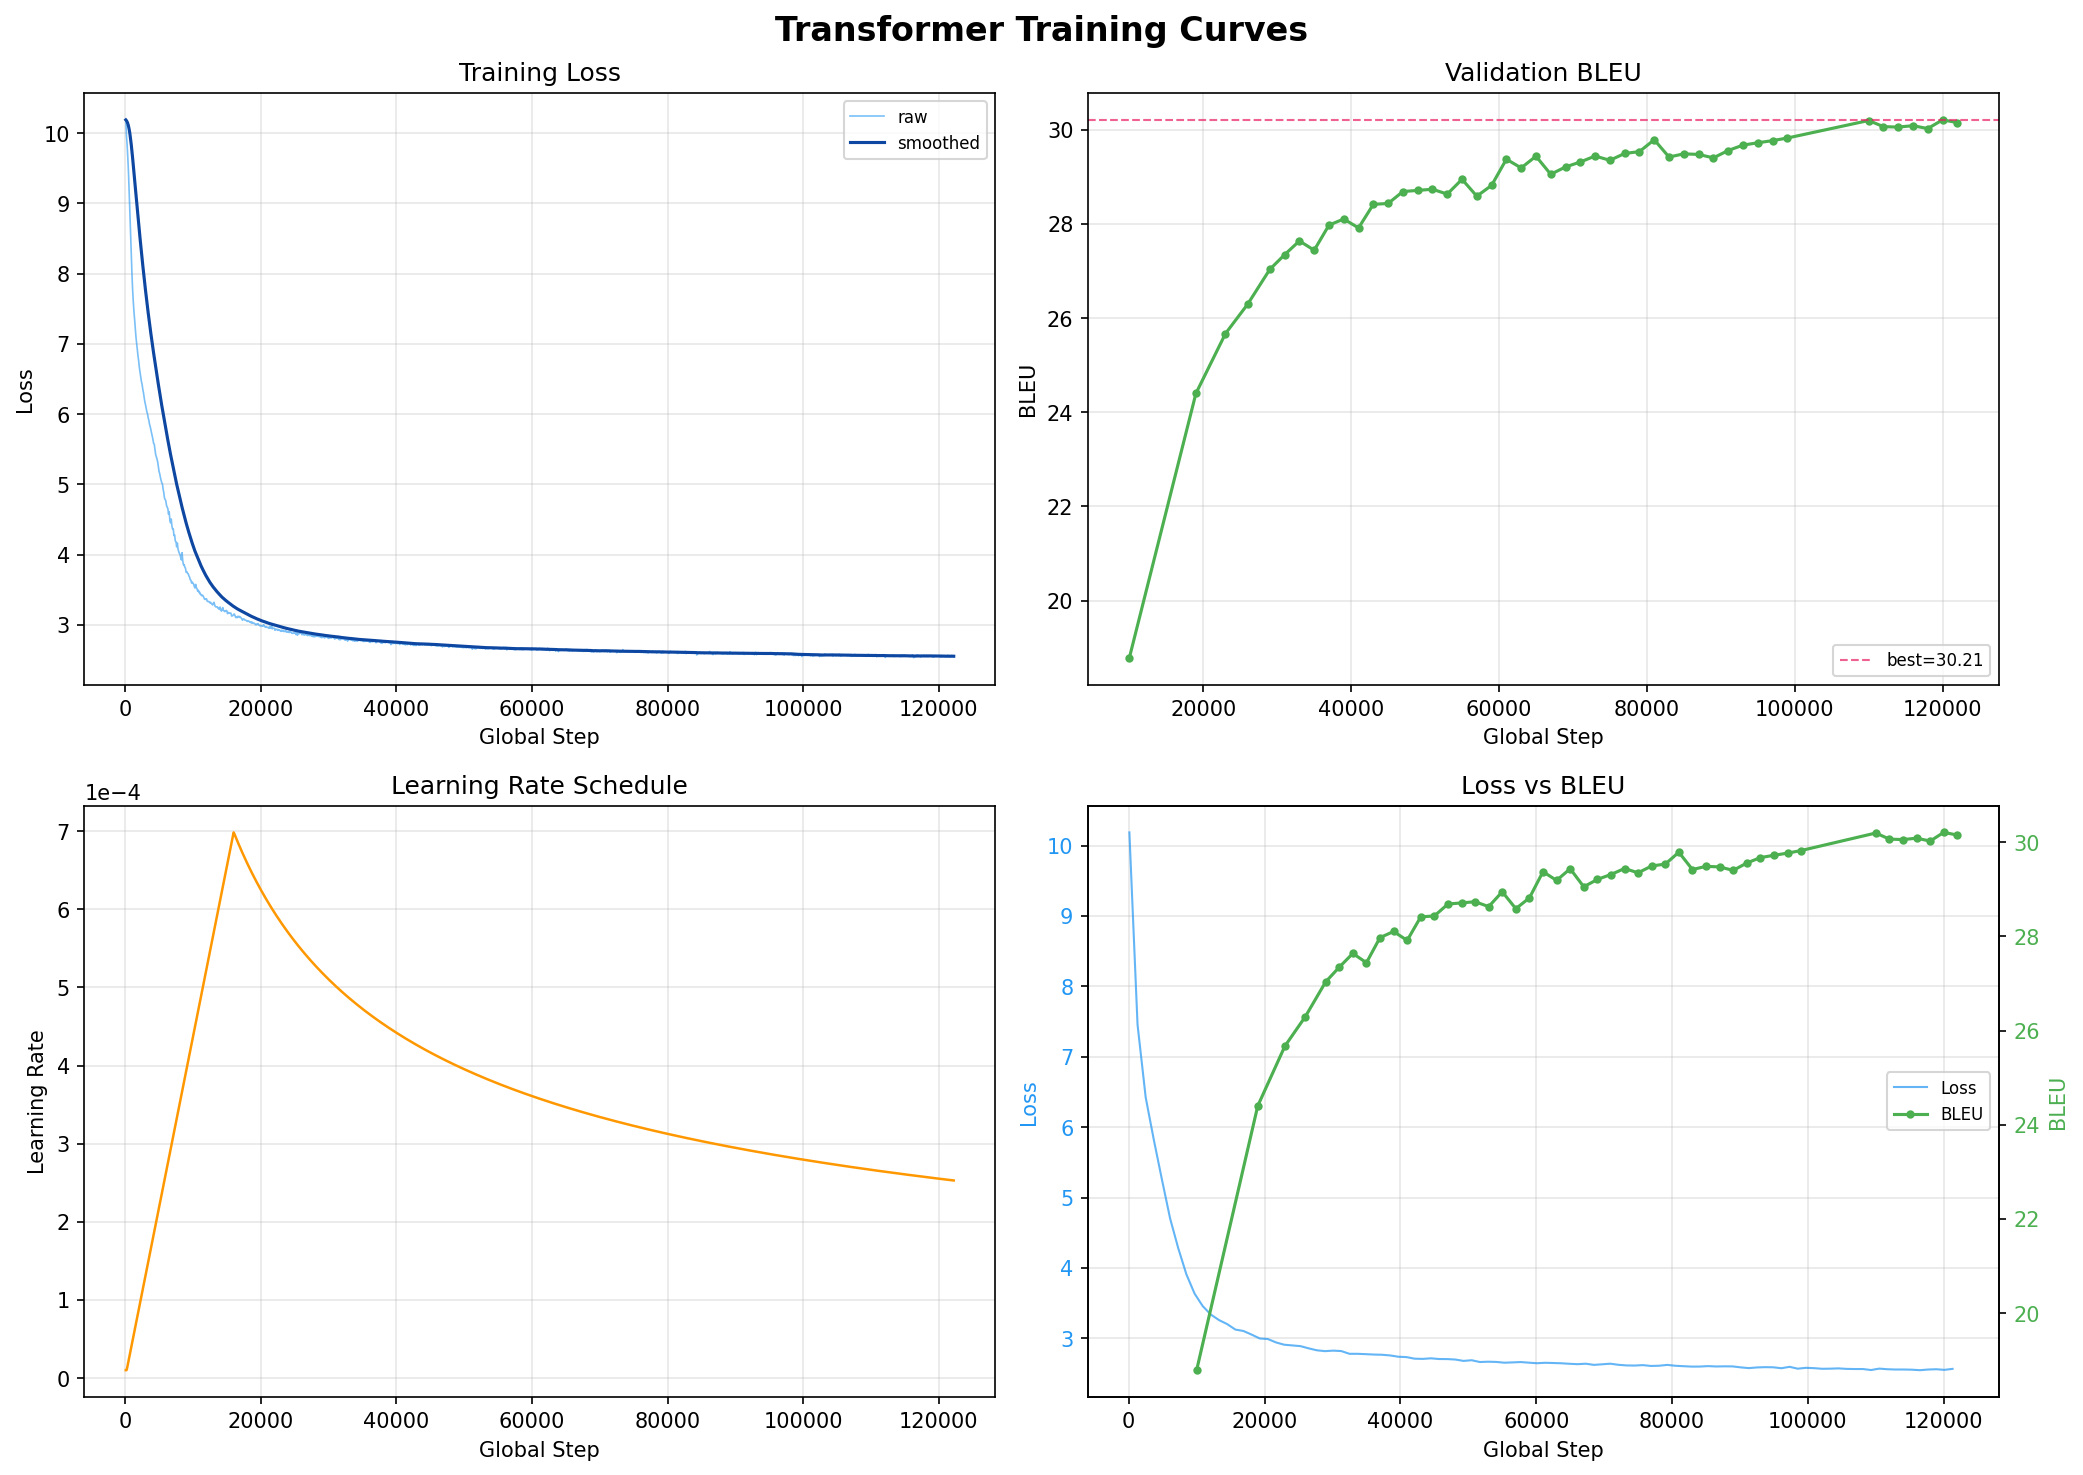
\includegraphics[width=\columnwidth]{figures/base_v1_curves.png}
\caption{Base v1.1 training curves (60M parameters, 122K steps, 9.3M strict-filter en-fr corpus). Top-left: training loss; top-right: validation BLEU (newstest2013) climbing monotonically through 30.21; bottom-left: Noam learning-rate schedule with peak $\approx 7\text{e-}4$ at warmup step 4K; bottom-right: loss/BLEU joint view. Zero spike-guard activations across the run.}
\label{fig:base_v1_curves}
\end{figure}

\subsection{Big v1.1: 209M parameters, same data}
\label{sec:big_v1}
Trained from scratch for 280K steps with the same data, SPM, and eval pipeline; early-stopped at 260K under patience. Best single-checkpoint valid is 30.69. Averaging 5 checkpoints in [210K, 250K] gives valid 31.14 / test 35.87. Total wall-clock: 6~h on the 5090.

\begin{figure}[t]
\centering
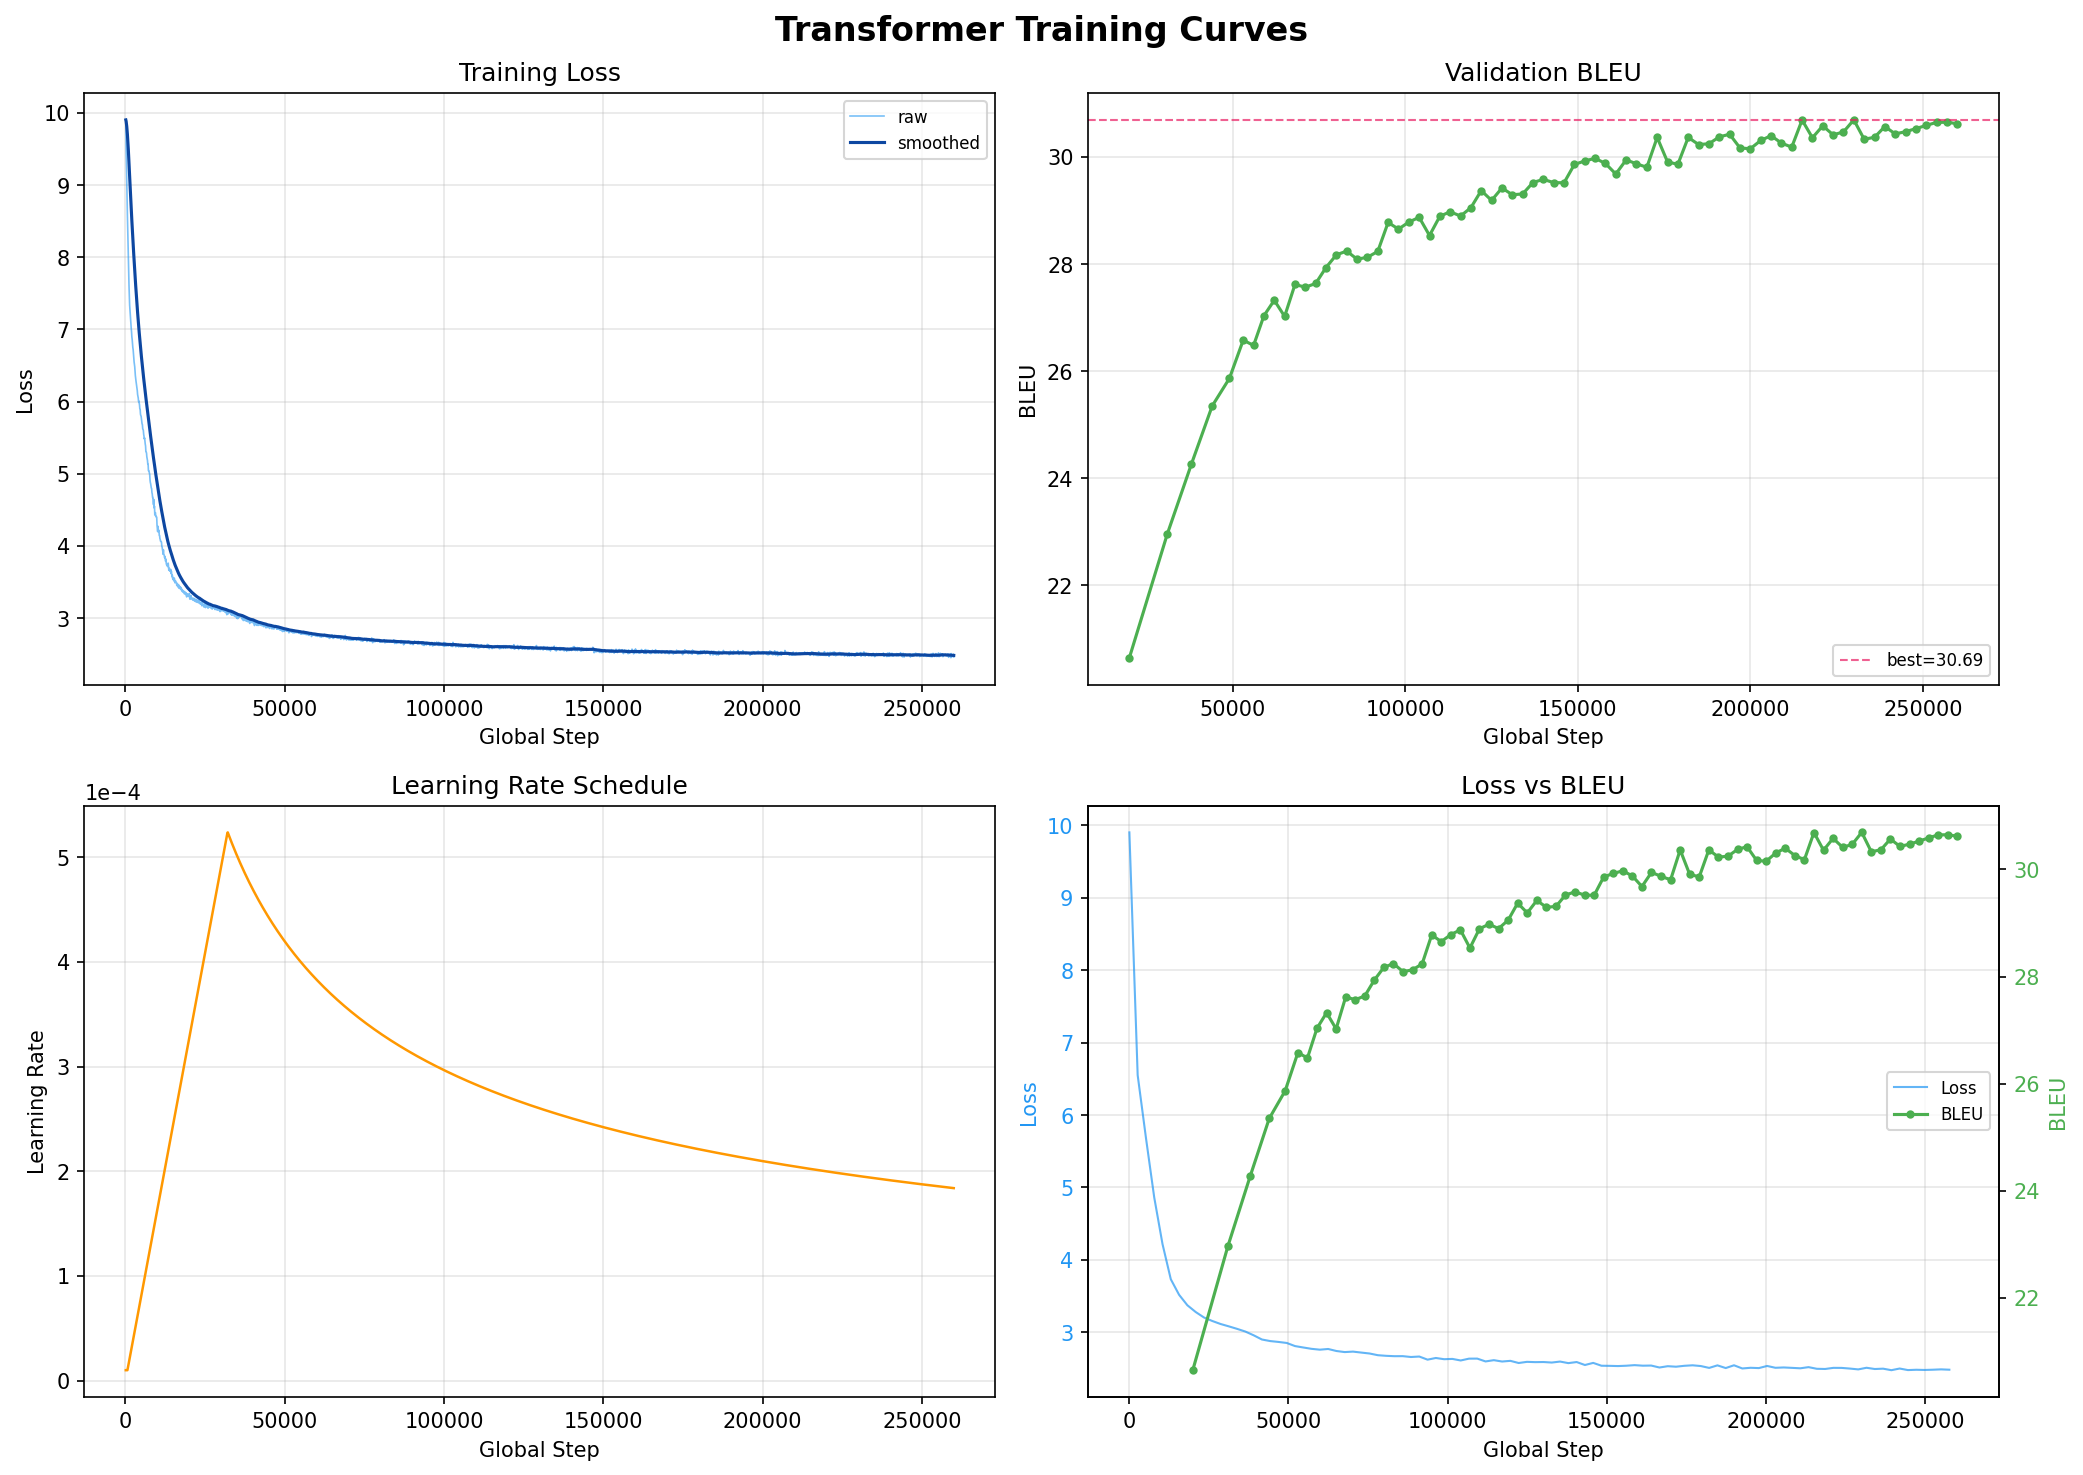
\includegraphics[width=\columnwidth]{figures/big_v1_curves.png}
\caption{Big v1.1 training curves (209M parameters, early-stopped at 260K of 280K planned, same 9.3M strict-filter en-fr corpus as Base v1.1). Validation BLEU plateaus around 30.5--30.7 from step 200K onwards; training-loss floor reaches $\sim$~2.3 (vs.\ Base v1.1's $\sim$~3.3). The lower loss floor at greater capacity is the data point exploited in \S\ref{sec:methodology}.}
\label{fig:big_v1_curves}
\end{figure}

\subsection{Capacity gap on clean data}
\label{sec:v1_capacity}

\begin{table}[t]
\centering
\small
\begin{tabular}{lrrr}
\toprule
\textbf{Run} & \textbf{Params} & \textbf{Valid} & \textbf{Test} \\
\midrule
Base v1.1 & 60M  & 30.52 & 35.31 \\
Big  v1.1 & 209M & 31.14 & 35.87 \\
\midrule
$\Delta$ (Big $-$ Base) & $+3.5\times$ & $+0.62$ & $\mathbf{+0.56}$ \\
\bottomrule
\end{tabular}
\caption{Capacity gap on the clean v1.1 corpus. BLEU on newstest2013 (valid) / newstest2014 (test); sacrebleu 13a, beam=5, length-penalty=1.0, 5-checkpoint averaged. Big exceeds Base by $+0.56$ BLEU on test.}
\label{tab:v1_capacity}
\end{table}

The $+0.56$ test gap is the ``capacity pays'' baseline of the 2x2. \S\ref{sec:enfr_v2} will show that on the loose-filter v2 corpus the same architectural change costs $-0.87$ BLEU, flipping the sign.

The gap is small in absolute terms compared to typical contemporary scaling reports, but it is consistent with the original paper's $\sim$~1 tokenized-BLEU Big-over-Base gap on en-fr (Vaswani 38.1 Big vs 37.0 Base $\approx$ +1.1 tokenized $\approx$ +0.5--0.7 sacrebleu). The relative scaling magnitude is preserved; the next section shows that this magnitude depends on the data being clean.

\subsection{Provenance: v1.0 numbers (retired)}
For reference: v1.0 (with \texttt{character\_coverage=0.9995}, 100K steps) reached test 34.69 (Base) / 34.66 (Big) --- the two sat within noise on the same data, which we initially interpreted as a ``shared tokenizer ceiling''. The v1.1 numbers (35.31 / 35.87) show that this was a tokenizer artifact rather than a capacity ceiling: with the tokenizer fixed, Big cleanly separates from Base. We retain v1.0 only as historical context; all subsequent analysis uses v1.1.

\section{Failure Case: en-fr on the Loose-Filter v2 Corpus}
\label{sec:enfr_v2}

This section reports the failure side of the 2x2 ablation. Base v2 and Big v2 share the pipeline, SPM, eval, and hyperparameters of their v1.1 counterparts; only the training corpus changes (v1's 9.3M strict-filter $\rightarrow$ v2's 30M loose-filter, drawn from the same WMT14 source pool). Both v2 runs converge cleanly. \emph{Both land below their v1 counterparts}, and \emph{Big v2 lands below Base v2} on identical data. The 2x2 closes here.

\subsection{Corpus construction}
v2 starts from the same WMT14 en-fr raw $\sim$~40.8M, cleaned with the same per-pair filters as v1, but \emph{without} the 10M-head cap. 30.1M pairs survive (74\% keep rate, vs.\ v1's 93\% on the head 10M). The 19-point keep-rate gap quantifies how much noisier the long tail is once the cap is removed.

A schedule re-tune is required because v2 is $3.2\times$ larger: Base v2 runs 600K steps (vs.\ Base v1.1's 122K) and Big v2 runs 800K (vs.\ Big v1.1's 280K), preserving the $\sim$~3-epoch budget. Warmup is scaled proportionally (4K~$\rightarrow$~12K for Base, 8K~$\rightarrow$~24K for Big). All other hyperparameters are unchanged.

\subsection{Base v2: 60M parameters, 30M loose data}
\label{sec:base_v2}
Trained for 600K steps (4 epochs over 30M); best converged valid is 28.66, and averaging 5 checkpoints gives valid 29.23 / test 33.90. Total wall-clock: $\sim$~14~h.

This sits \textbf{below Base v1.1} on both splits: $-1.29$ valid, $-1.41$ test. Despite seeing $3.2\times$ more data and running $4.9\times$ more optimizer steps, v2 underperforms v1.1 by more than a full BLEU.

\begin{figure}[t]
\centering
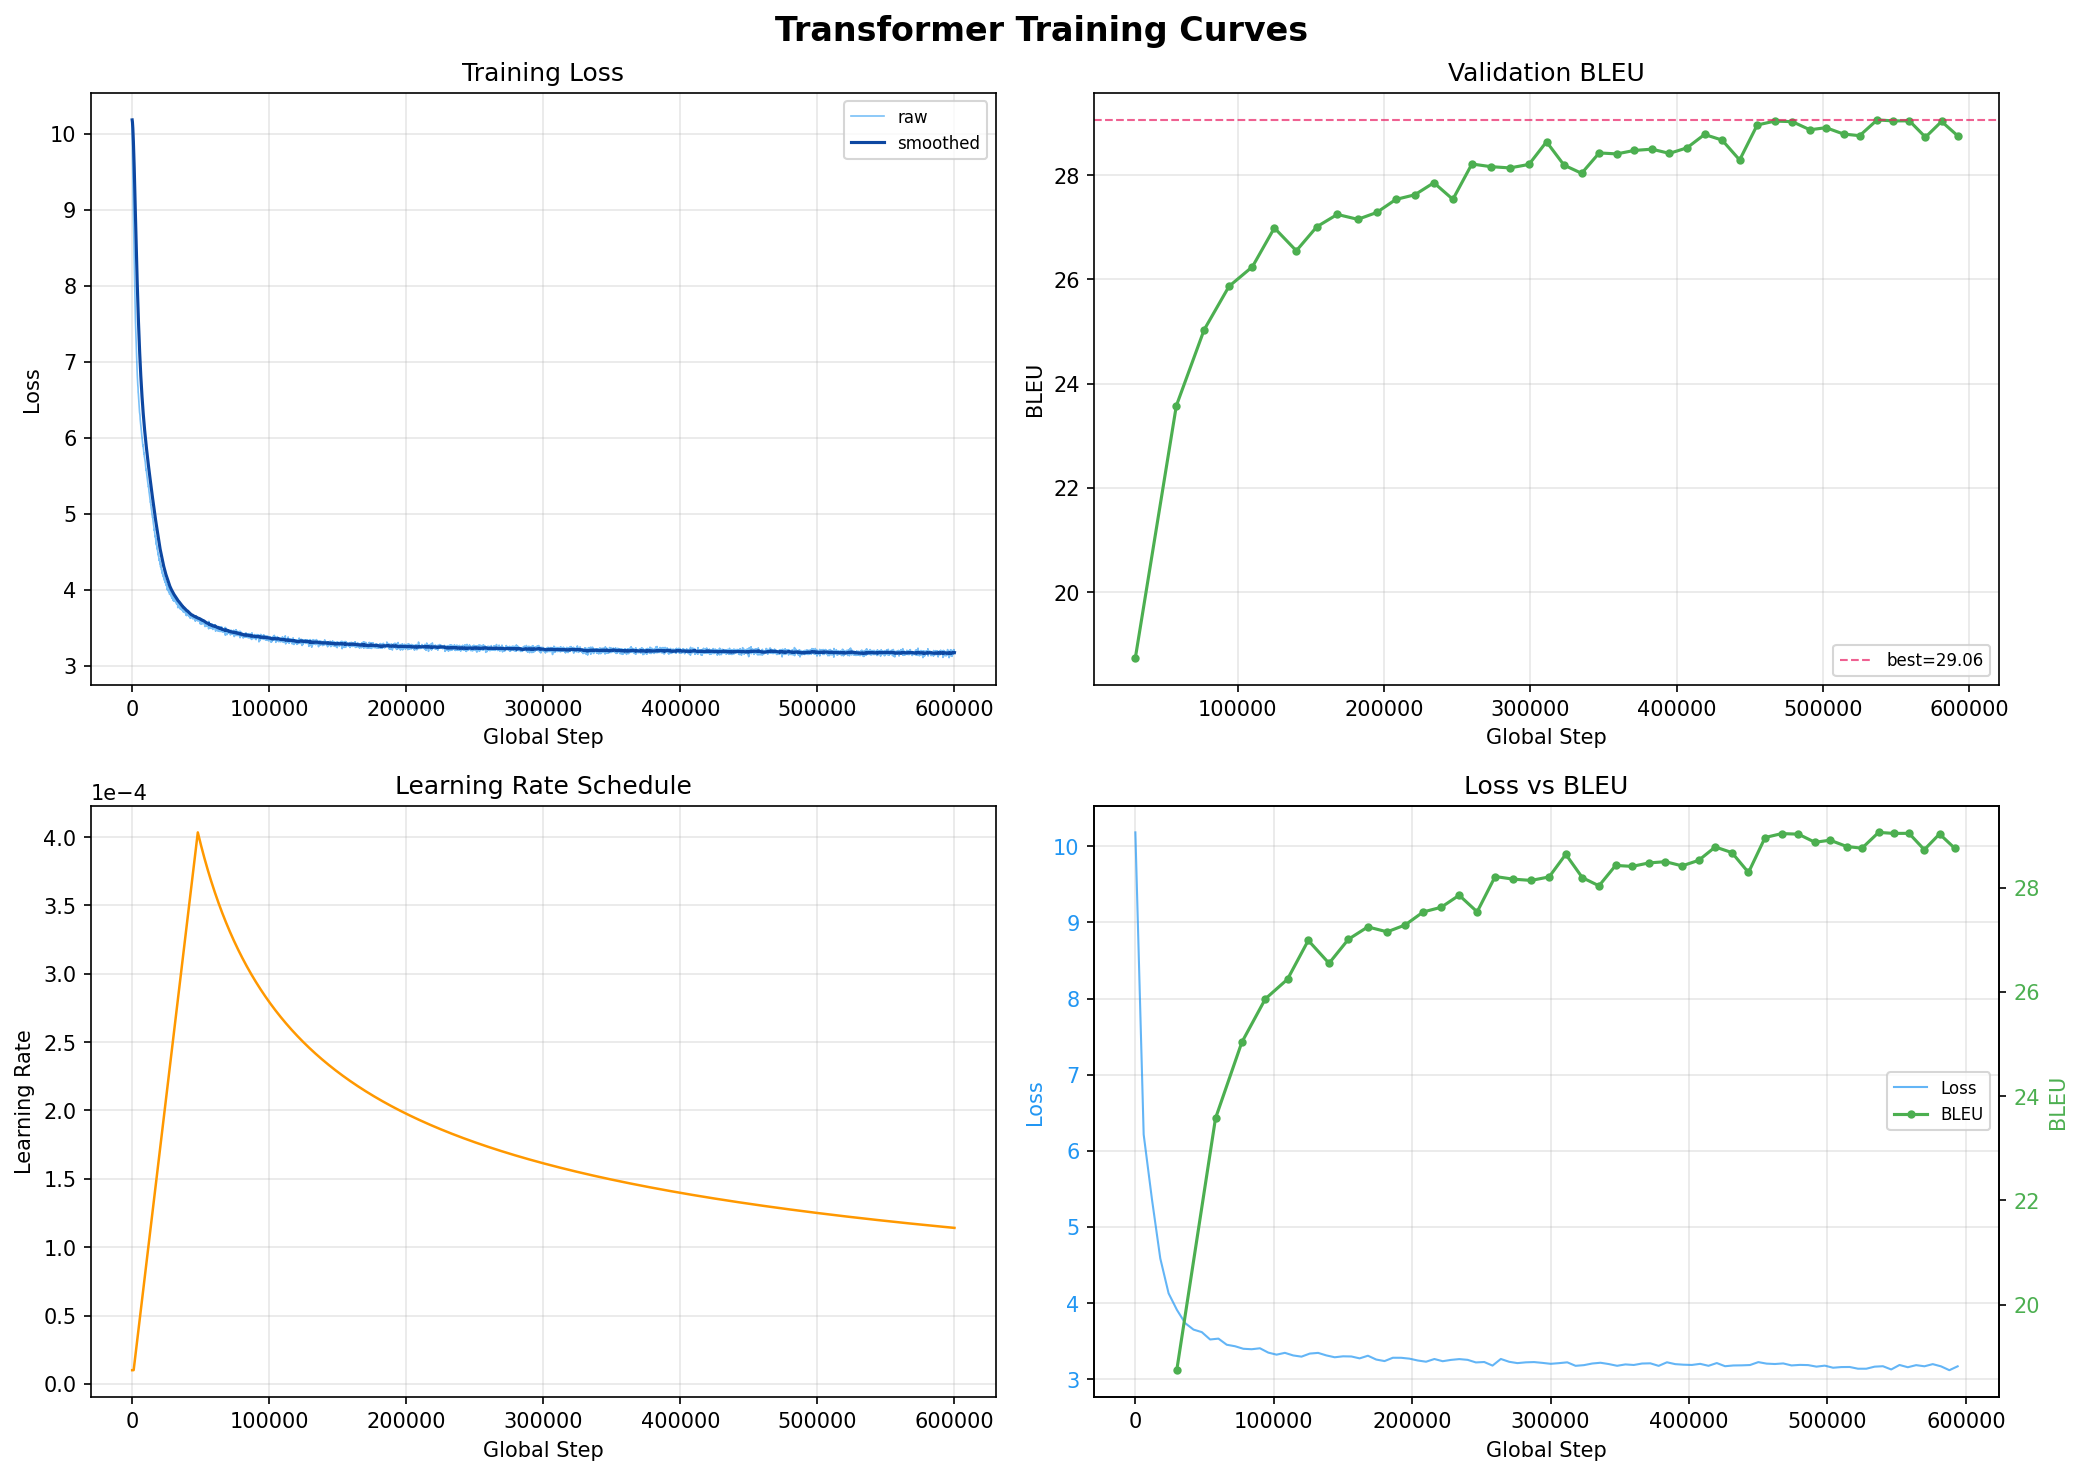
\includegraphics[width=\columnwidth]{figures/base_v2_curves.png}
\caption{Base v2 training curves (60M parameters, 600K steps, 30M loose-filter en-fr corpus). Loss converges smoothly; BLEU plateaus near 28.5--29 from step 400K onwards, $\sim$~1.4 below Base v1.1's averaged 30.52 baseline despite $4.9\times$ the optimizer steps and $3.2\times$ the data.}
\label{fig:base_v2_curves}
\end{figure}

\subsection{Big v2: 209M parameters, 30M loose data}
\label{sec:big_v2}
Trained from scratch for 800K planned steps; halted at 416K once valid BLEU plateaued and a single eval dipped below the running best. Best single-checkpoint valid is 27.77; averaging 5 checkpoints in [345K, 416K] gives valid 28.91 / test 33.03. Total wall-clock: $\sim$~9~h to halt.

This sits \textbf{below Base v2} on both splits: $-0.32$ valid, $-0.87$ test. The same $3.5\times$ extra parameters that paid $+0.56$ on v1 (\S\ref{sec:v1_capacity}) cost $-0.87$ here. The capacity gap has flipped sign.

\subsection{The 2x2 result}
\label{sec:two_by_two}

\begin{table}[t]
\centering
\small
\begin{tabular}{lrrr}
\toprule
\textbf{Data} & \textbf{Base (60M)} & \textbf{Big (209M)} & \textbf{$\Delta$} \\
\midrule
v1.1 (9.3M strict) & 35.31 & \textbf{35.87} & $\mathbf{+0.56}$ \\
v2 (30M loose)     & \textbf{33.90} & 33.03 & $\mathbf{-0.87}$ \\
\midrule
\textbf{Quality drop} & $-1.41$ & $-2.84$ & --- \\
\bottomrule
\end{tabular}
\caption{The 2x2 result: test BLEU on newstest2014; sacrebleu 13a, beam=5, length-penalty=1.0, 5-checkpoint averaged. Bold marks the better model within each row (capacity gap) and column (data-quality gap). The Big$-$Base difference flips sign: $+0.56$ on clean data, $-0.87$ on noisy data. Equivalently, the v1$\rightarrow$v2 quality drop is twice as large for Big ($-2.84$) as for Base ($-1.41$).}
\label{tab:two_by_two}
\end{table}

Table~\ref{tab:two_by_two} is the central empirical claim of the paper. Two ways to read it:
\begin{enumerate}
\item \textbf{Row-wise (capacity gap):} on clean data Big beats Base by $+0.56$; on noisy data Big falls below Base by $-0.87$. A single architectural change has opposite effects on opposite-quality data.
\item \textbf{Column-wise (data-quality drop):} both models lose BLEU on the noisier corpus, but Big loses twice as much ($-2.84$ vs.\ $-1.41$). Capacity does not absorb noise; it amplifies its cost.
\end{enumerate}

These are the same claim viewed two ways: capacity is a force multiplier whose sign depends on the supervision signal it is multiplying.

\subsection{Why v2 is noisy: direct evidence}
We attribute v2's degradation to noise in the extra 20M pairs beyond the v1 head 10M. Three pieces of supporting evidence:

\paragraph{Spike-guard activations.} The loss-spike guard (\S\ref{sec:setup}) fires when a batch's loss exceeds $1.3\times$ the EMA --- intended to drop pathologically wrong batches. On Base v1.1's 122K-step run it fires \textbf{0 times}; on Big v2's 416K-step run it fires \textbf{12 times} ($\approx$~1 per 35K steps). The 0-vs-nonzero contrast is the direct signal: clean v1 contains no batches that loss-spike a competent model, while v2 contains 12 such batches over its longer run. \S\ref{sec:methodology} adds a methodology caveat about cross-capacity spike-guard comparisons.

\paragraph{Sample inspection.} Manual inspection of the 100 lowest-scoring v2 pairs by CometKiwi-22 (``low'' in the 0.05--0.3 range) reveals the expected pathologies: source sentences echoed verbatim as ``translation'', misaligned pairs, repeated boilerplate from web-scraped UN documents, partial translations, and reverse-direction translations (fr~$\rightarrow$~en where en~$\rightarrow$~fr was expected). These pairs survive the per-pair length and ratio filters because those filters are token-counting heuristics and do not detect semantic misalignment.

\paragraph{Schedule was not the cause.} An earlier v2 attempt with 200K steps (a linear $2\times$ over v1's 100K) underfit badly --- training loss had not reached its v1 floor by the schedule end. We rejected that attempt and adopted 600K (a $4\times$ schedule for $3.2\times$ data, with proportional warmup), which trains to a tight loss floor. The headline 600K-step Base v2 result is post-convergence, not under-training.

\subsection{Big v2 was halted early: was that the right call?}
Big v2 was planned for 800K steps and halted at 416K. The halt rule: a single eval drops below the running best, AND the run has been pathologically slow to find new bests. At halt, Big v2's averaged BLEU was 33.03 / 28.91, already well below Base v2's 33.90 / 29.23 at the same wall-clock.

Could continued training to 800K have lifted Big v2 above Base v2? The trajectory in Figure~\ref{fig:big_v2_curves} makes this unlikely under the observed trend: late-training BLEU oscillates within $\pm 0.5$ around 27.7--28.0 from step 300K through 416K with no upward drift, while training loss plateaus at $\sim$~3.0. Further steps would have kept reducing loss on noisy patterns; we have no evidence they would have produced additional BLEU gain. We accept the halt as the conservative call and note that continued training could plausibly drift Big v2 further below 33.03 (more noise fitting) rather than above.

\begin{figure}[t]
\centering
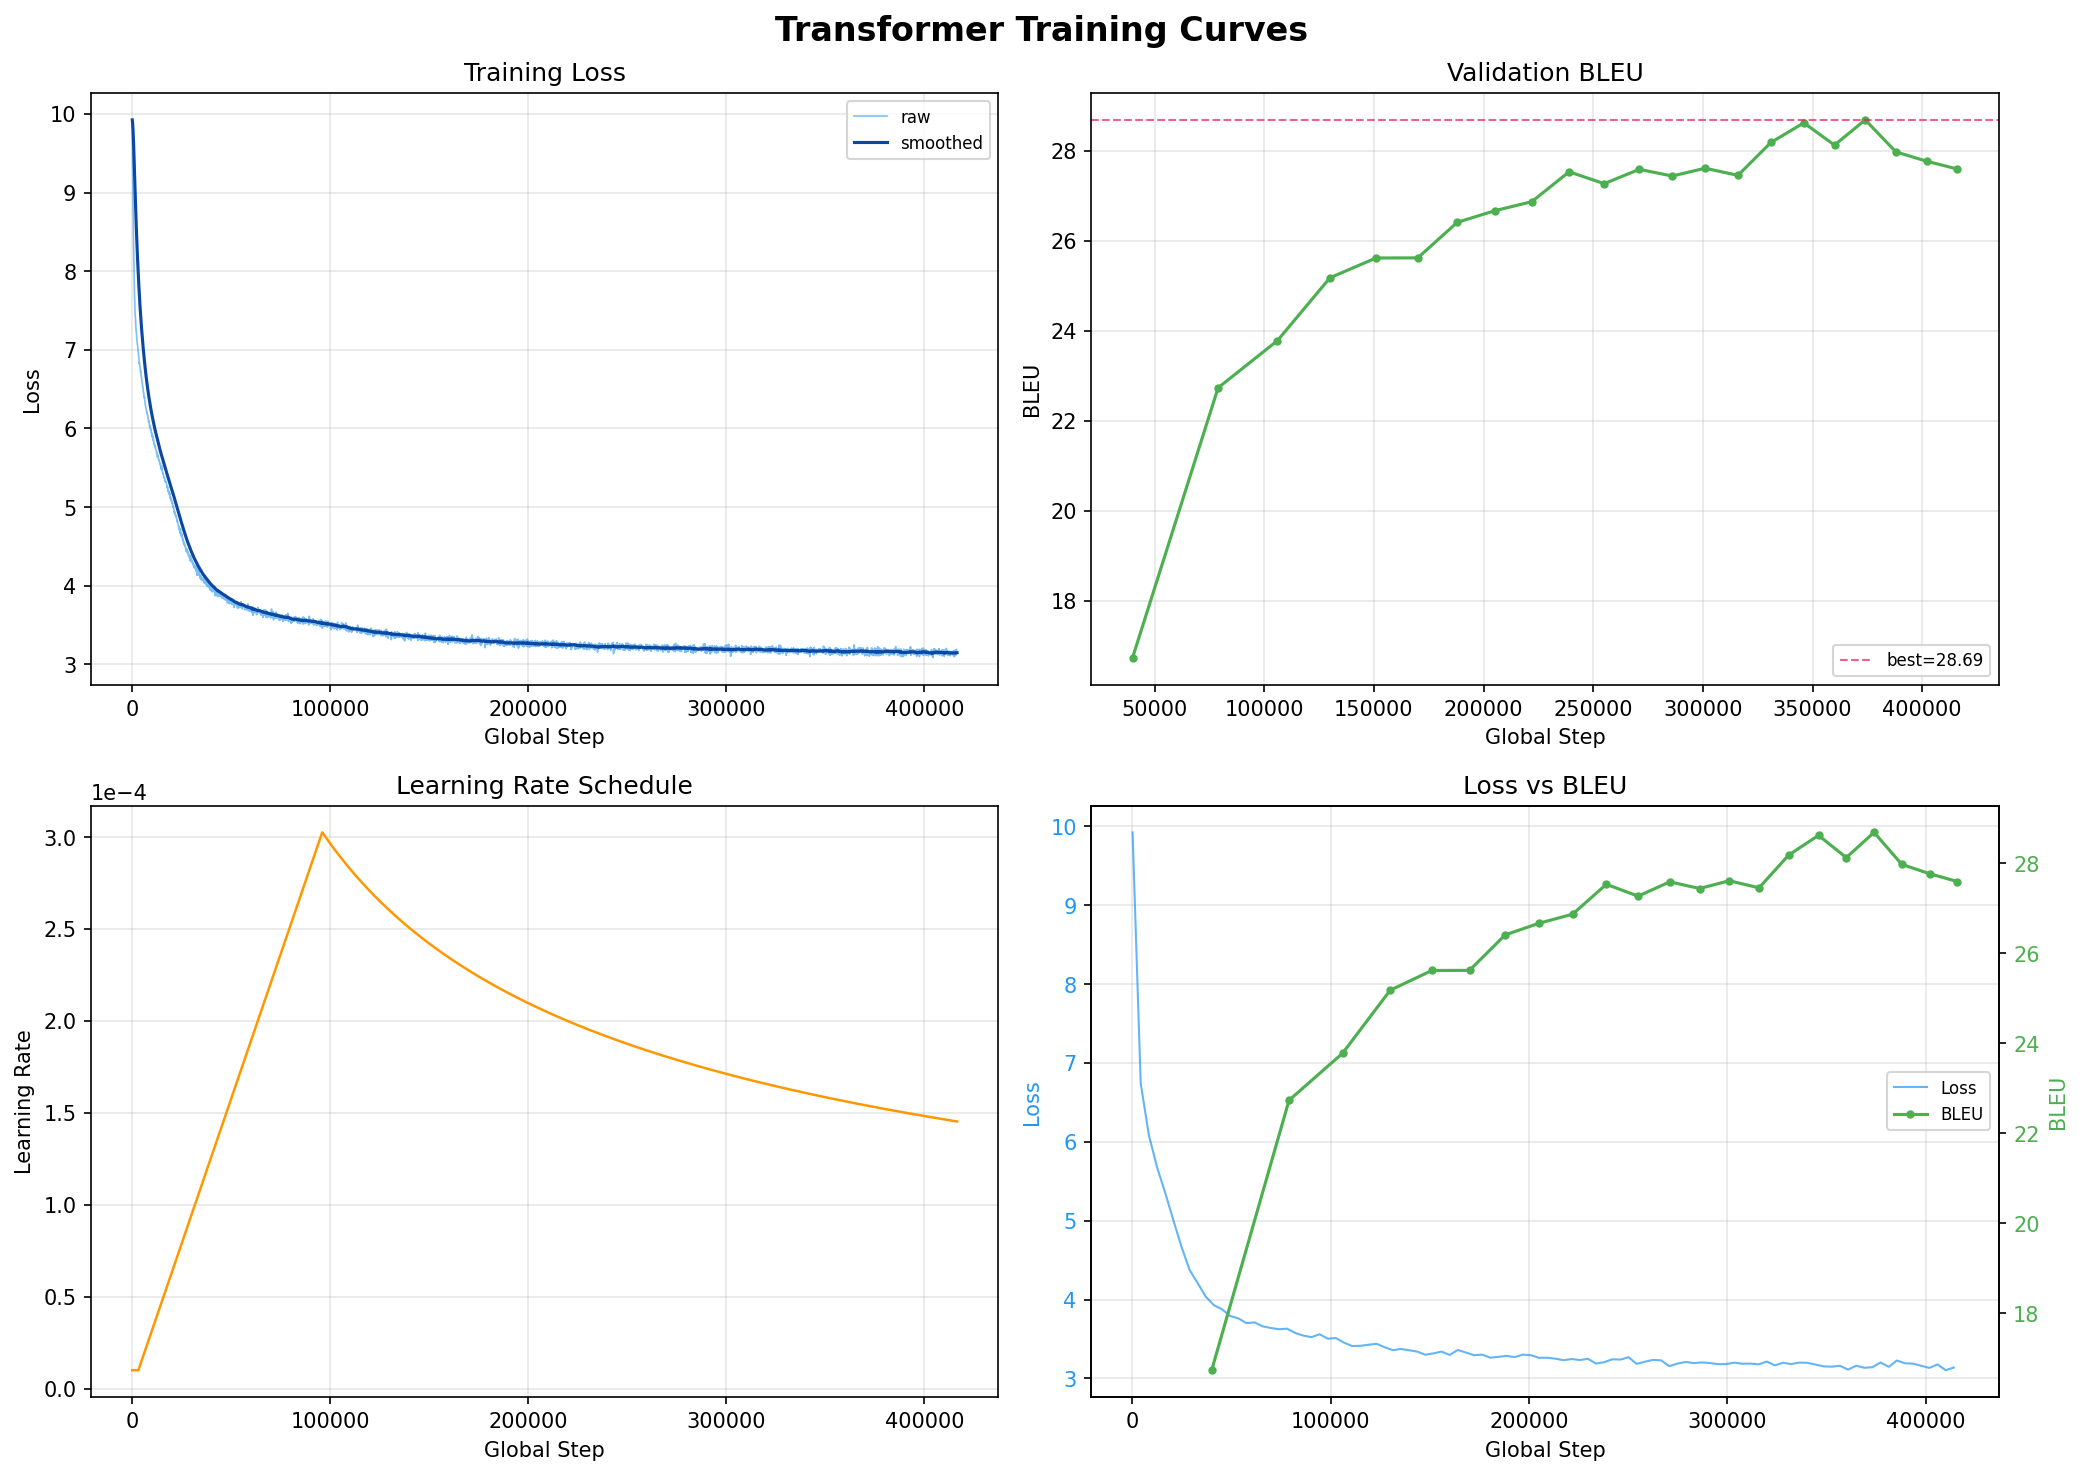
\includegraphics[width=\columnwidth]{figures/big_v2_curves.png}
\caption{Big v2 training curves (planned 800K, halted at 416K). Training loss converges smoothly to $\sim$~3.0; valid BLEU plateaus at 27.7--28.0 from step 300K onwards with no improving trend. The 12 spike-guard activations during this run are documented in \S\ref{sec:methodology}.}
\label{fig:big_v2_curves}
\end{figure}

\subsection{Combined prescription so far}
\S\ref{sec:enfr_v1}--\S\ref{sec:enfr_v2} together argue:

\begin{quote}
\textbf{Filter first, scale second.} Expanding v1$\rightarrow$v2 lowers BLEU for both models, with the larger losing more. The v1.1 capacity gap ($+0.56$) only emerges when the data is clean. Spending extra capacity on noisy data is counterproductive at this scale.
\end{quote}

\S\ref{sec:ende} replicates the pattern at smaller scale (4.5M pairs, en-de). \S\ref{sec:sft} then asks whether v2's noise can be removed after the fact via QE-filtered fine-tuning --- a natural follow-up that yields a different kind of failure.

\section{Cross-Language Replication: WMT14 en-de}
\label{sec:ende}

This section asks whether the en-fr 2x2 pattern generalizes to a different language pair. We pick WMT14 en-de --- a $4.5\times$ smaller raw corpus than en-fr (4.5M vs.\ 40.8M), where the raw data is already cleaner per-pair. The corpus is small enough that no clean v1/v2 split is possible (there is no ``loose'' option that yields meaningfully more data); instead we train a single Base and a single Big on the standard cleaned corpus and inspect the Base/Big gap.

\subsection{Corpus and setup}
WMT14 en-de is downloaded via HuggingFace Datasets (4{,}509{,}489 raw pairs) and cleaned with the v1 thresholds; 4{,}174{,}104 pairs survive (92.6\% keep rate). SPM 32K joint vocabulary, \texttt{character\_coverage=1.0} (preserves German umlauts). Train/valid/test $=$ 4.17M / 3{,}000 / 3{,}003.

Hyperparameters mirror the en-fr Base config (\S\ref{sec:setup}) with two changes: max\_steps 100K $\rightarrow$ 230K (extended after the curve at 150K showed continued non-trivial improvement), and dropout 0.1 $\rightarrow$ 0.3 for Big (following the original Vaswani recommendation for the smaller en-de corpus).

\subsection{Base en-de}
Base en-de trains for 230K steps ($\sim$~6 epochs at this batch size); best single-checkpoint valid is 24.25, and 5-checkpoint averaged valid / test reach 24.35 / 24.04 under default beam=5, lp=1.0. The original paper reports tokenized BLEU 27.3 on en-de Base; converting via the ${\sim}1.5$--$2$ tokenized-vs-sacrebleu band, our 24.04 sacrebleu corresponds to $\sim$~25.5--26 tokenized BLEU --- 1--1.5 BLEU below the original. Switching to the original en-de decoding hyperparameters (beam=4, lp=0.6) does not close the gap (24.19 sacrebleu, $+0.15$). The remaining gap is small relative to the $+0.56$ / $-0.87$ effects we make claims on, and likely reflects BPE tokenization and training-corpus filtering details that we cannot precisely reproduce.

\begin{figure}[t]
\centering
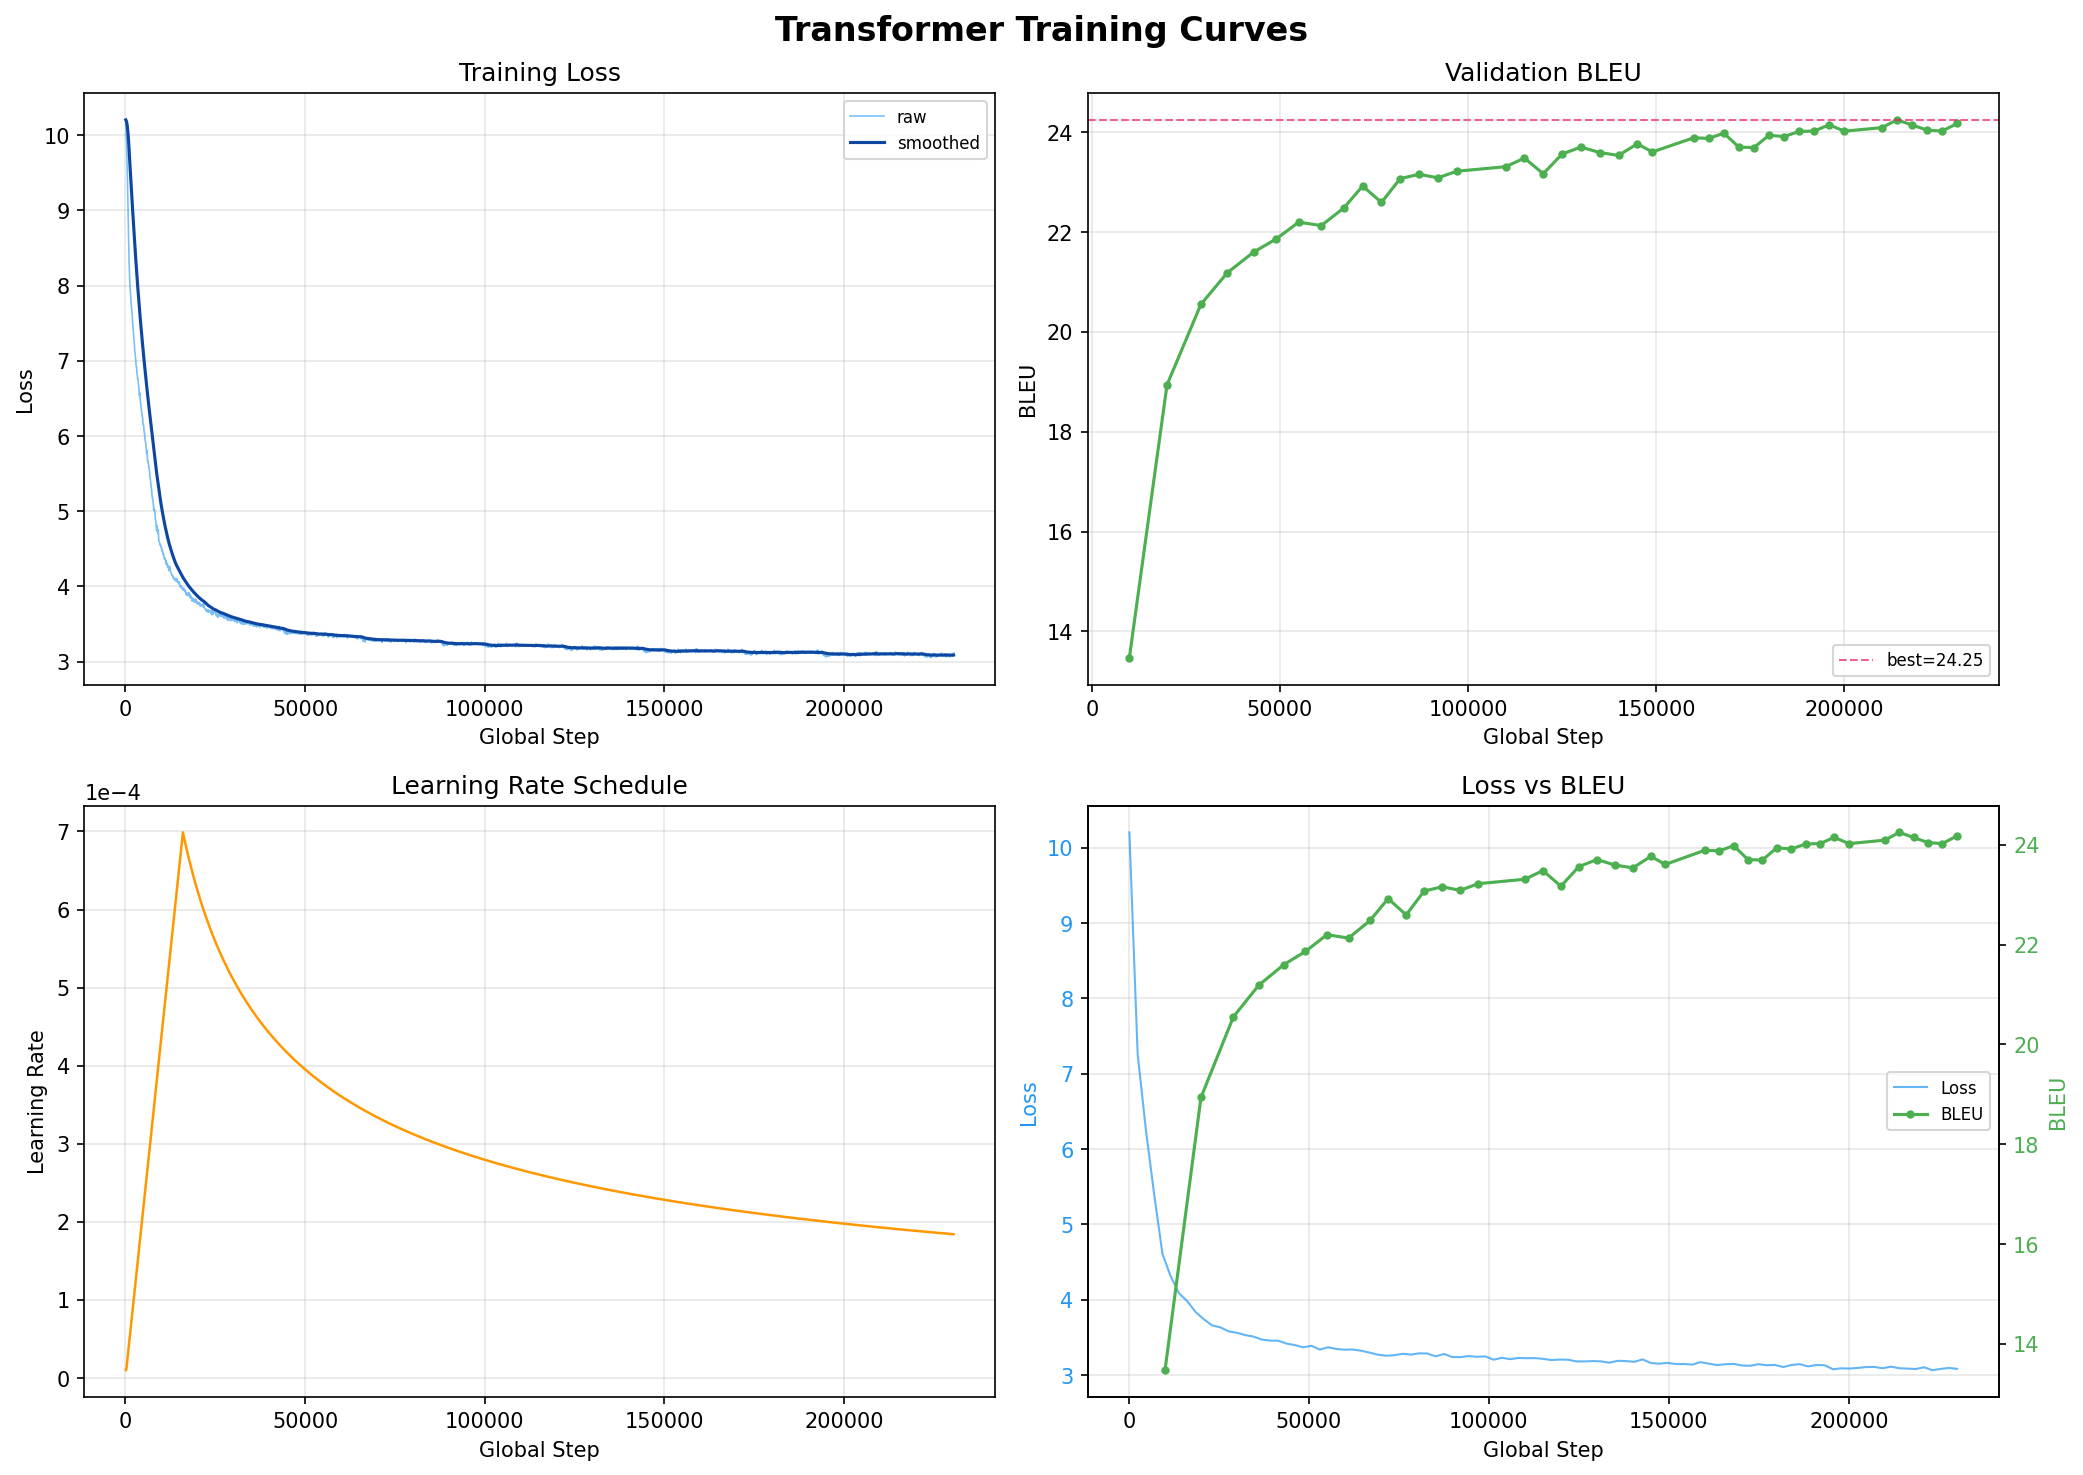
\includegraphics[width=\columnwidth]{figures/base_ende_curves.png}
\caption{Base en-de training curves (60M parameters, 230K steps, 4.17M strict-filter en-de corpus). Validation BLEU climbs monotonically through 24.25 by step 214K and plateaus thereafter. The valid/test gap is narrow (24.35 / 24.04 averaged, $-0.31$) consistent with newstest2013 and newstest2014 being similar-difficulty en-de news distributions.}
\label{fig:base_ende_curves}
\end{figure}

\subsection{Big en-de}
Big en-de trains for 466K steps with dropout 0.3 (the original Vaswani en-de regularization); best single-checkpoint valid is 23.41, with 5-checkpoint averaged valid / test 23.01 / 22.47.

\subsection{The pattern replicates}
\begin{table}[t]
\centering
\small
\begin{tabular}{lrrr}
\toprule
\textbf{en-de} & \textbf{Base (60M)} & \textbf{Big (209M)} & \textbf{$\Delta$ (Big$-$Base)} \\
\midrule
Valid & 24.35 & 23.01 & $-1.34$ \\
Test  & 24.04 & 22.47 & $\mathbf{-1.57}$ \\
\bottomrule
\end{tabular}
\caption{en-de results on newstest2013 (valid) / newstest2014 (test). sacrebleu 13a, beam=5, length-penalty=1.0, 5-checkpoint averaged. \textbf{Big falls below Base by $-$1.57 BLEU on test} and $-$1.34 on valid. The capacity gap is wider than en-fr v2's $-0.87$, consistent with --- but not necessarily caused by --- the smaller effective corpus.}
\label{tab:ende}
\end{table}

The Base $>$ Big ordering on en-de matches the direction of en-fr v2's $-0.87$, with a larger magnitude ($-1.57$ on test). The two may differ mechanistically: en-fr v2 fails through data \emph{noise}, while en-de plausibly fails through data \emph{quantity}, since 4.5M en-de is genuinely cleaner per-pair (\S\ref{sec:setup}) than 30M en-fr v2 yet $\sim$~half the size of clean v1.1's 9.3M. Both routes yield Base $\geq$ Big.

A unifying \emph{hypothesis} consistent with the three data points so far is that Big requires both (a) cleanly-aligned data and (b) enough of it: v1.1 has both, v2 has (b) but not (a), and en-de has (a) but not (b). Three points do not establish a curve, and we avoid claiming a precise scale threshold; we only note that the en-de result is consistent with this picture. A cross-language scaling sweep with multiple corpus-size points per language would be needed to test the hypothesis directly.

\subsection{HuggingFace release}
Both en-de checkpoints are published on the HuggingFace Hub:
\texttt{euswbnix/transformer-wmt14-ende-base} (60M, test 24.04) and
\texttt{euswbnix/transformer-wmt14-ende-big} (209M, test 22.47).

\section{Post-Training: QE-Filtered Fine-Tuning and the Multi-Dimensionality of ``Quality''}
\label{sec:sft}

\subsection{Motivation}
\S\S\ref{sec:enfr_v1}--\ref{sec:ende} establish a controlled 2x2: \textbf{data quality determines the sign of the capacity return}. On the strict-filter v1.1 corpus (9.3M pairs), Big exceeds Base by $+0.56$ BLEU; on the loose-filter v2 corpus (30M pairs), Big falls below Base by $-0.87$. The natural follow-up question is whether v2's extra 20M pairs are \emph{recoverable}: can we extract the high-quality subset of v2 and use it to push past v1.1's plateau?

This section tests that hypothesis with \emph{QE-filtered fine-tuning}: we score the full v2 corpus with a reference-free quality-estimation (QE) model, take the top-1M pairs by score, deduplicate, and continue training Base v1.1 and Big v1.1 on this filtered subset under the same cross-entropy loss as pretraining. \textbf{This is not instruction or preference tuning.}\footnote{We use ``fine-tuning'' (FT) in this section to denote continued pretraining-style training on a curated parallel-corpus subset. We avoid ``SFT'' alone because in the LLM literature it now most commonly refers to instruction tuning on (prompt, response) pairs, which is not the procedure here.} The intent is to retain whatever signal v2 contributes beyond v1's strict cutoffs while discarding the noise.

The outcome is a clean negative finding, and the negative finding is itself the contribution: it constrains what ``data quality'' means.

\subsection{Method}
\paragraph{Scoring.} We use CometKiwi-22 (\texttt{Unbabel/wmt22-cometkiwi-da})~\cite{rei2022cometkiwi}, the WMT22+ standard reference-free QE model based on XLM-RoBERTa-XL~\cite{conneau2020unsupervised}. Each $(\text{src}, \text{mt})$ pair receives a scalar quality score in roughly $[0, 1]$. Scoring v2's 30{,}129{,}500 pairs took 13.8 hours on a single RTX 5090 ($\approx$~750 pairs/sec at batch size 64), with scores concentrated in $[0.5, 0.92]$.

\paragraph{Filtering.} We retain the top 1M pairs by score (the top 3.3\% of v2). The retained band is tight --- 0.8959--0.9145 --- indicating a dense plateau of near-equivalent high-quality pairs above the cutoff.

\paragraph{Deduplication.} Sorting and unique-ing the top-1M yields 931{,}366 unique pairs (a 7\% duplicate rate, mostly UN-document boilerplate). All FT below uses this 931K-pair deduplicated set.

\paragraph{FT setup.} We fine-tune the averaged Base v1.1 and Big v1.1 checkpoints by resuming training with the optimizer state reset. The Noam scheduler resumes at post-warmup decay, giving an effective peak LR of $2.7\text{e--}4$ (Base) / $2.0\text{e--}4$ (Big) --- within the 10--20\% of pretraining-peak band conventional for FT. Other hyperparameters are unchanged from pretraining: bf16, label smoothing 0.1, eval every 2K steps. We allow up to 10K FT steps; both runs early-stop under default patience after $\approx$~6K steps.

\paragraph{Evaluation.} newstest2013 (valid) and newstest2014 (test), sacrebleu 13a, beam=5, length-penalty=1.0. We reuse the same SPM (coverage=1.0) from v1.1 pretraining.

\subsection{Results}
\label{sec:sft_results}

\textbf{Unit-of-comparison reminder.} The pretraining baselines we compare against are 5-checkpoint averages (Vaswani's averaging trick); the fine-tuning runs here are too short (6K steps) to produce 5 save-interval-spaced checkpoints, so their numbers come from single final checkpoints. Averaging the fine-tuning runs would likely add 0.2--0.4 BLEU. The reported $\Delta$s in Table~\ref{tab:sft_results} therefore overstate the fine-tuning loss by roughly that amount. The directional finding --- monotonic degradation, Big-loses-more-than-Base --- is unaffected.

BLEU decreases monotonically throughout fine-tuning on both models and both splits (Table~\ref{tab:sft_results}, Figure~\ref{fig:sft_curves}).

\begin{table}[t]
\centering
\small
\begin{tabular}{lrr}
\toprule
\textbf{Run} & \textbf{Test} & \textbf{Valid} \\
\midrule
Base v1.1 baseline (averaged) & 35.31 & 30.52 \\
Base v1.1 + FT (final ckpt)  & 33.77 \scriptsize{($-1.54$)} & 28.97 \scriptsize{($-1.55$)} \\
\midrule
Big  v1.1 baseline (averaged) & 35.87 & 31.14 \\
Big  v1.1 + FT (final ckpt)  & 33.54 \scriptsize{($-2.33$)} & 29.05 \scriptsize{($-2.09$)} \\
\bottomrule
\end{tabular}
\caption{QE-filtered fine-tuning degrades both Base and Big v1.1. BLEU on newstest2013 (valid) / newstest2014 (test); sacrebleu 13a, beam=5, length-penalty=1.0. Pretraining \emph{baselines} are 5-checkpoint averaged; \emph{fine-tuning} figures are single final checkpoints (6K-step runs did not produce 5 save-interval-spaced checkpoints; averaging would likely lift fine-tuning BLEU by 0.2--0.4, narrowing reported $\Delta$s by the same amount). Big loses more than Base by 0.5--0.8 BLEU on both splits.}
\label{tab:sft_results}
\end{table}

\begin{figure}[t]
\centering
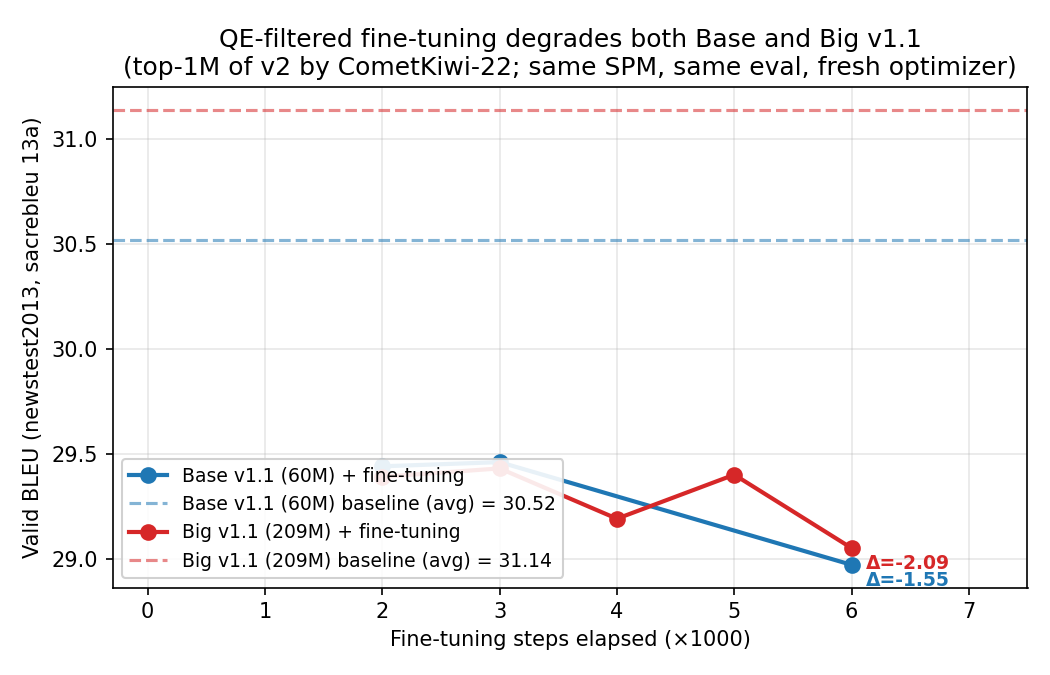
\includegraphics[width=\columnwidth]{figures/sft_curves.png}
\caption{Validation BLEU (newstest2013, sacrebleu 13a, beam=5, length-penalty=1.0) during QE-filtered fine-tuning. Solid lines are single-checkpoint evaluations during fine-tuning; dashed lines are pretraining baselines (5-checkpoint averaged). Both Base v1.1 (blue) and Big v1.1 (red) drop monotonically below their baselines. The first fine-tuning eval (step $+2$K) loses approximately 1 BLEU; subsequent steps drift further. Big drops more than Base.}
\label{fig:sft_curves}
\end{figure}

Training loss on the FT set converges smoothly from ${\sim}3.5$ (the pretraining floor on v1) to 1.94 (Base FT floor); the loss curve shows no sign of optimization failure. Sample translations during FT remain fluent and grammatically correct; accented French characters (\textit{Israël}, etc.) are preserved (no \texttt{<unk>}) thanks to the v1.1 SPM. \textbf{The drop is not a translation-quality collapse --- it is a distribution shift.}

Two observations from these numbers anticipate the analysis:
\begin{enumerate}
\item Big loses more than Base on both splits ($-0.79$ test, $-0.54$ valid). The architectural property that makes Big a better learner of clean in-distribution signal also makes it more pliable to whatever distribution it is fine-tuned on.
\item The FT-degraded models land near their v2-pretrained counterparts: Base$+$FT test 33.77 $\approx$ Base v2 test 33.90; Big$+$FT test 33.54 $>$ Big v2 test 33.03. Two genuinely different failure modes --- pretraining on noise (\S\ref{sec:enfr_v2}) and FT under a domain-mismatched filter (\S\ref{sec:sft}) --- converge to the same 33--34 BLEU band. We argue in \S\ref{sec:why_failures_differ} that this is not coincidence.
\end{enumerate}

\subsection{Why the filter selected what it did}
CometKiwi-22 is reference-free: it scores translation quality in absolute terms. The top-5 highest-scored pairs after deduplication are dominated by UN, intergovernmental, and legislative parallel data --- long, formal, syntactically rigid sentences with statistical content, professionally translated (Table~\ref{tab:top5_samples}).

\begin{table*}[t]
\centering
\small
\begin{tabular}{p{0.5cm} p{6.5cm} p{6.5cm} p{2cm}}
\toprule
\# & Source (en) & Translation (fr) & Domain \\
\midrule
1 & \emph{It is estimated that there are 500--650 million persons with disabilities in the world, approximately 10\% of the world population, 150 million of whom are children.} & \emph{On estime qu'il y a entre 500 et 650 millions de personnes handicapées dans le monde, soit environ 10\% de la population mondiale; 150 millions d'entre elles sont des enfants.} & UN report \\
\addlinespace
2 & \emph{The estimated number of people living with HIV in Eastern Europe and Central Asia rose to 1.5 million in 2007; almost 90\% of those infected live in either the Russian Federation (69\%) or Ukraine (29\%).} & \emph{On estime que le nombre de personnes vivant avec le VIH en Europe orientale et en Asie centrale a atteint 1,5 million en 2007; près de 90\% des personnes infectées vivent soit en Fédération de Russie (69\%) soit en Ukraine (29\%).} & UNAIDS \\
\addlinespace
3 & \emph{Since 2005--2006, the Government has reduced the federal debt by \$37 billion.} & \emph{Depuis 2005--2006, le gouvernement a réduit la dette fédérale de 37 milliards de dollars.} & Gov. \\
\addlinespace
4 & \emph{During 2006, the population of Finland increased by 4 per cent (21,375 persons).} & \emph{En 2006, la population finlandaise a augmenté de 4\,\% (21\,375 personnes).} & Stat. \\
\bottomrule
\end{tabular}
\caption{Top-4 highest-scoring v2 pairs by CometKiwi-22 (after deduplication; score band 0.8959--0.9145). The top scorers are professionally-translated UN/intergovernmental/legislative documents; WMT14 newstest is news domain.}
\label{tab:top5_samples}
\end{table*}

This is unsurprising: such corpora exhibit the alignment, completeness, and syntactic correspondence that QE is trained to reward. WMT14 newstest, in contrast, is news-domain --- looser register, shorter sentences, conversational interjections, named-entity-rich, with occasional ungrammaticality from quoted speech.

We thus have two distributions: an FT distribution (high-quality, formal, document-style) and an eval distribution (high-quality, informal, news-style). FT pulls the model's output distribution toward the former. On the FT distribution itself the model improves; on the eval distribution it gets worse, because every FT step trades news-style fit for formal-style fit.

\textbf{The model is not deteriorating in absolute quality.} It is being relocated in distribution space, and that relocation moves it away from the eval distribution.

\subsection{Implication: ``data quality'' decomposes}
This negative result refines the central claim of the paper:
\begin{quote}
Capacity return is determined by data quality. \emph{(\S\ref{sec:enfr_v1}--\S\ref{sec:ende})}
\end{quote}
\S\ref{sec:sft} forces a decomposition of ``quality'':
\begin{quote}
\textbf{Data quality = (translation correctness) x (alignment to target distribution).}
Both dimensions matter, and they are independent. Reference-free QE metrics measure the first; they do not measure the second.
\end{quote}

A naive top-K-by-QE filter optimizes only the first axis, and on a heterogeneous corpus (which v2 is --- news, web, UN, Europarl, all mixed) this can move the data far from the target eval distribution. The cleaner the QE filter, the more pronounced the domain skew, because high-quality parallel data is disproportionately UN/legislative.

This generalizes: any post-training step that filters on absolute quality without conditioning on the eval distribution risks moving the model away from where it should land. The fix is not ``better QE'' --- CometKiwi-22 is doing exactly what it should --- but \emph{domain-conditional filtering}: filter by QE within news-domain candidates, sample uniformly across domains within a QE band, or apply a domain classifier as a hard pre-filter.

\subsection{Why the v2-pretraining failure and the FT failure are different mechanisms}
\label{sec:why_failures_differ}

It is worth distinguishing the two failure modes the paper has now exhibited (Table~\ref{tab:two_failures}).

\begin{table}[t]
\centering
\small
\begin{tabular}{p{2.4cm} p{2.4cm} p{2.4cm}}
\toprule
& v2 pretraining (\S\ref{sec:enfr_v2}) & FT (\S\ref{sec:sft}) \\
\midrule
Data & all 30M v2 (noisy) & top-1M (clean) \\
Mechanism & wrong supervision & wrong distribution \\
Big$-$Base $\Delta$ & $-0.87$ & $-0.79$ (test) \\
Lesson & filter for noise & match for distribution \\
\bottomrule
\end{tabular}
\caption{Two failure modes producing $\sim$~33--34 test BLEU on newstest2014. Both amplify with capacity at comparable magnitude. The Big$-$Base $\Delta$ row reports test-BLEU differences (sacrebleu 13a, beam=5, lp=1.0; pretraining figures averaged, fine-tuning figures single ckpt as in Table~\ref{tab:sft_results}).}
\label{tab:two_failures}
\end{table}

These failures are independent axes. CometKiwi-based quality filtering \emph{does} address the v2 noise problem --- inspection of low-scored v2 pairs confirms that genuine noise concentrates at the bottom of the distribution --- but it does not address the distribution-alignment problem, because high-quality translations exist in many domains and our top-K selector does not condition on domain.

\textbf{Both failure modes appear to amplify with capacity.} Big v2 falls below Base v2 by 0.87 (noise amplification); Big FT falls below Base FT by $0.54$--$0.79$ (distribution-shift amplification). A reading consistent with current evidence: the architectural property --- more parameters, more representational capacity --- that makes Big a better learner of correct supervision on clean in-distribution data also makes it a more efficient absorber of incorrect supervision and a more pliable conformer to whatever distribution it is fine-tuned on. Under this reading, capacity acts as a force multiplier whose sign depends on the data, not on the model. With $n{=}1$ seed per cell, we frame this as a hypothesis supported by the four data points we report, not an established mechanism.

\subsection{Limitations}
\begin{itemize}
\item \textbf{Single seed.} Variance in FT outcomes is small relative to the $-1.55$ to $-2.33$ effects, but a 3-seed mean would tighten the bound.
\item \textbf{No low-LR FT.} A peak LR $\leq 5\text{e--}5$ might find a ``shallow FT'' point that improves UN-style without hurting newstest. We expect the effect to scale with effective FT distance from baseline; very-low-LR FT is slow to test, and the paper's claim does not require it.
\item \textbf{No domain-conditional filtering.} Building a news-conditioned top-K filter is a nontrivial sub-project (domain classifier $+$ quality scorer $+$ joint sampling). We flag it as the natural fix and leave it to future work.
\end{itemize}

\subsection{Headline}
Quality-filtered FT, on its own, does not improve newstest BLEU when ``quality'' is measured by reference-free QE on a multi-domain corpus. It costs 1.5--2.3 BLEU on Base / Big v1.1. The cause is not filter failure --- the filter selected genuinely high-quality pairs --- but that absolute translation quality and alignment to the eval distribution are independent axes of ``quality'', and only the first was optimized. The negative result tightens the paper's prescription:

\begin{quote}
\textbf{Filter first (for noise), match the evaluation distribution second (for register/domain), and only then scale capacity.} Skipping the second step undoes the capacity returns from the first.
\end{quote}

\section{Methodology Note: Spike-Guard Trigger Rate is Not a Pure Noise Meter}
\label{sec:methodology}

We added a loss-spike guard (\S\ref{sec:setup}) to the trainer to drop pathologically high-loss batches: if the current batch's average loss exceeds $1.3\times$ an EMA of recent batches, the gradient is discarded. The guard exists for a defensive reason --- preventing a single mis-scraped pair from corrupting weights --- and we initially read its trigger rate as a clean diagnostic of \emph{data noise}. That reading was wrong. This section documents the corrected interpretation and the evidence behind it.

\subsection{Trigger counts across runs}

\begin{table}[t]
\centering
\small
\begin{tabular}{lrrr}
\toprule
\textbf{Run}                 & \textbf{Skips} & \textbf{Steps} & \textbf{per 10K steps} \\
\midrule
Base v1.1 (clean 9.3M)       & 0   & 122K & 0.00 \\
Big  v1.1 (clean 9.3M)       & 25  & 260K & 0.96 \\
Big  v2   (noisy 30M)        & 12  & 416K & 0.29 \\
\bottomrule
\end{tabular}
\caption{Spike-guard triggers across three runs, all using the same $1.3\times$ EMA threshold. Naively reading these as data-noise counts produces the surprising result that Big on \emph{clean} data triggers $3.3\times$ more often than Big on \emph{noisy} data. (Base v2 was an earlier run whose stdout logs were not retained; its trigger count is unrecoverable.)}
\label{tab:spike_rates}
\end{table}

If the guard rate were a pure data-noise metric, Big v1.1 (clean) and Big v2 (noisy) should differ in the obvious direction. Table~\ref{tab:spike_rates} shows the \emph{opposite}: at fixed Big capacity, the clean run triggers more often than the noisy run.

\subsection{The mechanism: tight-EMA false positives}

The guard threshold is $1.3\times$ \emph{the model's own EMA loss}. On clean data Big converges to a very low loss (training floor $\sim$~2.3), and the EMA tracks this floor tightly; even modest natural batch-to-batch variation can exceed $1.3\times$ a tight floor and trigger the guard. Triggered batches in this regime are essentially \emph{false positives} --- the model's well-converged baseline makes ordinary batches look spiky.

On noisy data the loss never converges as tightly: the noise floor stays elevated ($\sim$~3.0 for Big v2, vs.\ Big v1.1's $\sim$~2.3). The EMA is therefore looser, and only \emph{genuinely catastrophic} samples can exceed $1.3\times$ a higher floor. Triggers are rarer, but each one is more likely to be real.

The same mechanism therefore produces \emph{more triggers on cleaner data}, because cleanliness tightens the loss EMA and lowers the absolute spike-detection threshold.

\subsection{What can the trigger rate be used for?}

The corrected reading: \textbf{trigger rate is a joint function of data noise AND the model's own convergence depth.} Two implications:

\paragraph{Same-capacity, different-data comparisons are valid.} Base v1.1 vs.\ Base v2 is a clean test of data noise --- the model is fixed, only the data changes, so differences in trigger rate isolate to the data. Unfortunately the Base v2 stdout was not retained at training time, so we cannot report this comparison numerically. \emph{Our published v1.1 trainer now persists trigger counts to the training report so future runs are not lost.}

\paragraph{Cross-capacity, same-data comparisons are confounded.} Base v1.1 (0 triggers) and Big v1.1 (25 triggers) on identical data is \emph{not} evidence about the data --- it is evidence about the difference in convergence depth between the two models. Larger models reach lower loss floors, tightening their EMAs and inflating trigger counts on the \emph{same} corpus.

\paragraph{Same-capacity, same-data comparisons across runs} (e.g.\ comparing trigger rates from a tokenizer-fix retraining against the original) are valid as a sanity check that pipeline changes have not introduced new pathological samples.

\subsection{Recommendation}

For papers that wish to use spike-guard-style or RHO-Loss-style EMA-relative loss filters as a quantitative data-noise diagnostic, we recommend reporting the trigger rate \emph{conditional on convergence depth}, e.g.\ as a function of late-training EMA loss. We do not do this here: our trigger counts inform our intuition about v2 noise but are not a numeric claim. The 0-vs-12 Base v1.1 vs.\ Big v2 comparison we initially used in our project notes is confounded along two axes (different model, different data) and is superseded by the table above with its associated caveat.

This is a supplementary finding and does not affect the headline 2x2 claim. We include it because spike-guard or RHO-Loss-style~\cite{mindermann2022prioritized} filters are increasingly common in practice, and the false-positive-on-clean-data property is, in our experience, easy to miss until one accidentally produces a number that violates expectations.

\section{Conclusion}
\label{sec:conclusion}

We constructed a 2x2 ablation of data quality and model capacity in from-scratch Transformer machine translation, and found that the capacity return changes sign with data quality: $+0.56$ test BLEU on the strict-filter 9.3M en-fr corpus, $-0.87$ on the loose-filter 30M corpus drawn from the same source. The same architectural change pays in one regime and costs in another. The data-quality dimension qualitatively replicates on en-de at 4.5M scale (Base $>$ Big by 1.57 BLEU), supporting an interpretation under which Big requires both clean data \emph{and} enough of it; failing either condition flips the sign of the capacity return.

A natural follow-up --- can we recover v2's noise via post-training quality filtering? --- yields a clean negative result. Reference-free QE-filtered fine-tuning (CometKiwi-22, top-1M of the 30M v2 corpus, 6K fine-tuning steps under cross-entropy loss) degrades newstest BLEU by 1.5--2.3 on both Base and Big v1.1, with Big losing more. The mechanism is distinct from the noise-amplification of \S\ref{sec:enfr_v2}: the fine-tuning data is high-quality but heavily UN/legislative, mismatched to news domain. We argue that this decomposes ``data quality'' into translation correctness and target-distribution alignment --- two independent axes, of which reference-free QE measures only the first.

The paper's prescription, in three steps:
\begin{enumerate}
\item \textbf{Filter for noise.} Cap data at the strict-cleaning frontier; do not chase scale past the noise wall.
\item \textbf{Match the eval distribution.} QE-filtered fine-tuning or distillation \emph{must} condition on domain or register; absolute QE on its own is insufficient and can hurt.
\item \textbf{Then scale capacity.} The capacity return is $+0.56$ when (1) and (2) hold, and is negative or near zero when either fails.
\end{enumerate}

We close with a methodology caveat about loss-spike-guard trigger rates as a data-noise diagnostic: trigger rates are joint functions of data noise and model convergence depth, and only same-capacity / different-data comparisons are clean. Cross-capacity comparisons that we relied on in early drafts of this work were retroactively invalidated by this realization; the corrected analysis is in \S\ref{sec:methodology}.

\paragraph{What we did not test.}
Only two language pairs (en-fr, en-de). Single seed per configuration. No human evaluation. No back-translation augmentation. No domain-conditional QE filter --- the natural fix for the fine-tuning failure of \S\ref{sec:sft}, and the most concrete future-work direction. All checkpoints, code, configs, and stdout logs are released to enable independent replication.

\paragraph{What we hope is taken from this paper.}
The headline empirical claim: one cannot read off the value of extra capacity without knowing what data it will see, and one cannot read off the value of more data without knowing whether the post-training pipeline will move the model in the right direction. ``More data'' and ``more parameters'' are conditioned on each other and on the post-training pipeline. The 2x2 design we used --- {strict, loose} x {Base, Big}, on a shared source pool, with cross-language replication and a closed-loop fine-tuning test --- is itself a transferable template. We hope future scaling-and-data papers report it more often than they currently do.


\bibliographystyle{plain}
\bibliography{references}

\end{document}
